% I seguenti commenti speciali impostano:
% 1. utf8 come codifica di input,
% 2. PDFLaTeX come motore di composizione;
% 3. Articolo.tex come documento principale;
% 4. il controllo ortografico italiano per l'editor.

% !TEX encoding = UTF-8
% !TEX TS-program = pdflatex
% !TEX root = Articolo.tex
% !TEX spellcheck = it-IT

\documentclass[12pt,%                       % corpo del font principale
               a4paper,%                    % carta A4
               oneside,%                    % solo fronte
%  \={a}            twoside,%                    % fronte-retro
               ]{article}                  % classe report di KOMA-Script;
               
\usepackage[T1]{fontenc}                    % codifica dei font:
                                            % NOTA BENE! richiede una distribuzione *completa* di LaTeX,
                                            % per esempio TeXLive o MiKTeX *complete*

\usepackage[utf8]{inputenc}                 % codifica di input; anche [latin1] va bene
                                            % NOTA BENE! va accordata con le preferenze dell'editor

\usepackage[english,italian]{babel}         % per scrivere in italiano e in inglese;


\usepackage[binding=5mm]{layaureo}          % margini ottimizzati per l'A4; rilegatura di 5 mm

\usepackage{indentfirst}                    % rientra il primo capoverso di ogni sezione
\usepackage{booktabs}                       % tabelle
\usepackage{tabularx}                       % tabelle di larghezza prefissata
\usepackage{multirow}
\usepackage{graphicx}                       % immagini
\usepackage{subfig}                         % sottofigure, sottotabelle
\usepackage{pslatex}
\usepackage{wrapfig}
\usepackage{epsfig}
\usepackage{epstopdf}
\usepackage{textcomp}
% \usepackage{microtype}
\usepackage{caption}                        % didascalie
\usepackage{listings}                       % codici
\usepackage[font=small]{quoting}            % citazioni

\usepackage{amsmath,amssymb,amsthm}         % matematica

\usepackage[italian]{varioref}              % riferimenti completi della pagina

\usepackage{mparhack,fixltx2e,relsize}      % finezze tipografiche
\usepackage{braket}

\usepackage[backend=biber,style=authoryear-comp]{biblatex}
                                            % eccellente pacchetto per la bibliografia;
                                            % produce uno stile di citazione autore-anno; 
                                            % lo stile "numeric-comp" produce riferimenti numerici
                                          
\bibliography{Bibliografia}                 % database di biblatex 
                                          
\usepackage[svgnames]{xcolor}             % colori

\usepackage{hyperref}                       % collegamenti ipertestuali

\usepackage{bookmark}                       % segnalibri

\usepackage{xinttools}% for expandable and non-expandable loops
\usepackage[scaled]{beramono}
\usepackage{chngpage}
% \usepackage{tgheros}

%*********************************************************************************
% impostazioni-articolo.tex
% di Lorenzo Pantieri (2012)
% file che contiene le impostazioni dell'articolo
%*********************************************************************************


%*********************************************************************************
% Comandi personali
%*******************************************************
\newcommand{\myName}{Iuri La Rosa, Federico Muciaccia}                            % autore
\newcommand{\myTitle}{Antenna network breakdown}  % titolo
\date{}                                                           % nessuna data

\title{\myTitle}
\author{\myName}



%*********************************************************************************
% Impostazioni di amsmath, amssymb, amsthm
%*********************************************************************************

% comandi per gli insiemi numerici (serve il pacchetto amssymb)
\newcommand{\numberset}{\mathbb} 
\newcommand{\N}{\numberset{N}} 
\newcommand{\R}{\numberset{R}} 

% un ambiente per i sistemi
\newenvironment{sistema}%
  {\left\lbrace\begin{array}{@{}l@{}}}%
  {\end{array}\right.}

% definizioni (serve il pacchetto amsthm)
\theoremstyle{definition} 
\newtheorem{definizione}{Definizione}

% teoremi, leggi e decreti (serve il pacchetto amsthm)
\theoremstyle{plain} 
\newtheorem{teorema}{Teorema}
\newtheorem{legge}{Legge}
\newtheorem{decreto}[legge]{Decreto}
\newtheorem{murphy}{Murphy}[section]



%*********************************************************************************
% Impostazioni di biblatex
%*********************************************************************************
\defbibheading{bibliography}{%
\phantomsection 
\addcontentsline{toc}{section}{\refname}
\section*{\bibname\markboth{\MakeUppercase{\refname}}{\MakeUppercase{\refname}}}}



%*********************************************************************************
% Impostazioni di listings
%*********************************************************************************
\addto\captionsitalian{%
\renewcommand{\lstlistingname}{Snippet}}

\addto\captionsitalian{%
\renewcommand{\lstlistlistingname}{Elenco degli snippet}}

\lstset{language=[GNU]C++,
	basicstyle=\small\ttfamily,
	keywordstyle=\color{Black}\bfseries,
	identifierstyle=\color{Black},
	commentstyle=\color{Black},
	stringstyle=\color{Red}\ttfamily,
	numbers=none,
	numberstyle=\scriptsize,
	tabsize=4,
	stepnumber=1,
	numbersep=8pt,
	showstringspaces=false,
	breaklines=true,
	frame=single
% 	keywords=[2]{def}
%     emphstyle=\color{Goldenrod}
} 



%*********************************************************************************
% Impostazioni di hyperref
%*********************************************************************************
\hypersetup{%
    hyperfootnotes=false,pdfpagelabels,
    %draft,	% = elimina tutti i link (utile per stampe in bianco e nero)
    colorlinks=true, linktocpage=true, pdfstartpage=1, pdfstartview=FitV,%
    % decommenta la riga seguente per avere link in nero (per esempio per la stampa in bianco e nero)
    %colorlinks=false, linktocpage=false, pdfborder={0 0 0}, pdfstartpage=1, pdfstartview=FitV,% 
    breaklinks=true, pdfpagemode=UseNone, pageanchor=true, pdfpagemode=UseOutlines,%
    plainpages=false, bookmarksnumbered, bookmarksopen=true, bookmarksopenlevel=1,%
    hypertexnames=true, pdfhighlight=/O,%nesting=true,%frenchlinks,%
    urlcolor=webbrown, linkcolor=RoyalBlue, citecolor=webgreen, %pagecolor=RoyalBlue,%
    %urlcolor=Black, linkcolor=Black, citecolor=Black, %pagecolor=Black,%
    pdftitle={\myTitle},%
    pdfauthor={\textcopyright\ \myName},%
    pdfsubject={},%
    pdfkeywords={},%
    pdfcreator={pdfLaTeX},%
    pdfproducer={LaTeX with hyperref and ClassicThesis}%
}



%*********************************************************************************
% Impostazioni di graphicx
%*********************************************************************************
\graphicspath{{Immagini/}} % cartella dove sono riposte le immagini



%*********************************************************************************
% Impostazioni di xcolor
%*********************************************************************************
\definecolor{webgreen}{rgb}{0,.5,0}
\definecolor{webbrown}{rgb}{.6,0,0}



%*********************************************************************************
% Impostazioni di caption
%*********************************************************************************
\captionsetup{tableposition=top,figureposition=bottom,font=small,format=hang,labelfont=bf}



%*********************************************************************************
% Altro
%*********************************************************************************

% [...] ;-)
\newcommand{\omissis}{[\dots\negthinspace]}

% eccezioni all'algoritmo di sillabazione
\hyphenation{Fortran ma-cro-istru-zio-ne nitro-idrossil-amminico}               % file con le impostazioni personali
\begin{document}
\pagestyle{headings}
%******************************************************************
% Materiale iniziale
%******************************************************************
% %aumentato il carattere a 12 punti (prima era i 11)
\documentclass[a4paper,titlepage,twoside,openright]{book}
\usepackage[italian]{babel}
\usepackage[utf8]{inputenc}
\usepackage{pslatex}
\usepackage{epsfig}
%aggiunti per funzionare con eepic
%\usepackage{eepic,epic,eepicemu}
\usepackage{color}
% per grafici in latex come sopra
%\usepackage{longtable}
\usepackage{graphicx}
\usepackage{latexsym}
\usepackage{epstopdf}
\usepackage{microtype}%migliora la resa dei caratteri
% \usepackage[pdftex]{hyperref}
\usepackage{booktabs}
\usepackage{caption}
\usepackage{listings}
\usepackage{subfig}
\usepackage{wrapfig}
\usepackage{multirow}
\usepackage{amsmath,amssymb}
\usepackage{textcomp}
\usepackage[]{frontespizio}

\begin{document}

\begin{frontespizio}
	\Istituzione{ }
	\Logo{../Immagini/Sigillo}
	\Facolta{Scienze MM. FF. NN.}
	\Corso[Laurea Magistrale]{Fisica}
	\Annoaccademico{2015-2016}
	\Titoletto{Relazione per il corso di Sistemi Complessi}
	\Titolo{Antenna network breakdown}
% 	\Sottotitolo{Un'analisi generale sulle stelle di materia degenere}
	\Candidato{Iuri La Rosa}
	\Candidato{Federico Muciaccia}
	\NCandidati{Autori}
	\Relatore{Vittorio Loreto}
	\Relatore{Andrea Capocci}
	\NRelatore{Docente}{Docenti}
\end{frontespizio}

\end{document}

\newpage
% !TEX encoding = UTF-8
% !TEX TS-program = pdflatex
% !TEX root = ../Articolo.tex
% !TEX spellcheck = it-IT

%*******************************************************
% Sommario+Abstract
%*******************************************************
\phantomsection
\pdfbookmark{Sommario}{Sommario}
\section*{Sommario}

Lo scopo di questo lavoro è fare un'analisi di rete usando un campione di antenne telefoniche cellulari, ipotizzando di voler costruire una ipotetica *mesh network* con esse. Abbiamo scelto di analizzare il sistema delle antenne comprese entro il Raccordo Anulare di Roma. Non sapendo a priori di quale tipo di rete si tratta, e che tipo di grafo si costruisce da essa, sono state studiate alcune proprietà topologiche e comportamentali dell'insieme di antenne studiate.
Dopo aver definito il criterio con cui dare un link a due nodi, sono state calcolate le matrici di adiacenza della rete complessiva e di quelle composte solo dalle antenne dei singoli gestori presenti in Italia. La prima parte dell'analisi consiste nell'estrapolare dai grafi ottenuti le distribuzioni dei gradi e nell'affidare all'istogramma dei gradi la forma funzionale che meglio gli si adatti. Avendo così ottenuto indicazioni significative sui tipi di rete in analisi, le abbiamo verficate studiando il comportamento percolativo della rete, mediante rimozione di nodi in due diversi scenari: un attacco intenzionale, che rimuovesse le antenne a partire da quelle con maggior grado, e una caduta random del sistema. I risultati ottenuti sono stati confrontati con modelli di rete esponenziali e scale-free.
L'esposizione è articolata nel seguente modo:

\begin{description}
\item[{\hyperref[sec:teoria]{Nella sezione \ref{sec:teoria}}}] verranno esposte le basi teoriche dello studio effettuato, con particolare accento ai modelli di rete utilizzati come riferimento e ai concetti di percolazione e soglia percolativa.

\item[{\hyperref[sec:dati]{Nella sezione \ref{sec:dati}}}] si spiega come sono stati raccolti e organizzati i dati, come è stata definita la rete e quindi con quali criteri è stata definita la matrice di adiacenza. Successivamente, accennando ai problemi computazionali avuti nel gestire la rete complessiva da circa 7000 nodi, verranno calcolate le matrici di adiacenza e le distribuzioni del grado.

\item[{\hyperref[sec:attaack]{Nella sezione \ref{sec:attaack}}}] viene effettuato lo studio percolativo mediante i due scenari di rimozione di nodi,  analizzando l'andamento del diametro e delle dimensioni del cluster più grande con la progressiva caduta delle antenne. I risultati sono stati confrontati con quelli ottenuti dai modelli, i quali hanno rivelato delle ambiguità. Nel caso di attacco random è stato testato infine un ipotetico effetto cascata causato dall'overload delle antenne rimaste (previa rimozione dei grossi hub che servono proprio a scongiurare tale evenienza).

\end{description}


\newpage
% !TEX encoding = UTF-8
% !TEX TS-program = pdflatex
% !TEX root = ../Articolo.tex
% !TEX spellcheck = it-IT

%*******************************************************
% Indici
%*******************************************************
\pdfbookmark{\contentsname}{tableofcontents}
\setcounter{tocdepth}{2}
\tableofcontents
\markboth{\contentsname}{\contentsname} 
\clearpage
%*******************************************************
% Elenco delle figure
%*******************************************************    
\phantomsection
\pdfbookmark{\listfigurename}{lof}
\listoffigures
% \clearpage
%*******************************************************
% Elenco delle tabelle
%*******************************************************
% \phantomsection
% \pdfbookmark{\listtablename}{lot}
% \listoftables
% \clearpage        

\newpage


%******************************************************************
% Materiale principale
%******************************************************************
% !TEX encoding = UTF-8
% !TEX TS-program = pdflatex
% !TEX root = ../Relazione.tex
% !TEX spellcheck = it-IT

%%%%%%%%%%%%%%%%%%%%%%%
\section{Reti \emph{scale-free}}
\label{sec:teoria}
%%%%%%%%%%%%%%%%%%%%%%%
Le reti sono insiemi di oggetti per i quali è possibile una connessione. Gli ultimi 60 anni hanno visto un crescente interesse per esse, perché con le reti è possibile descrivere sistemi dei più disparati tipi nei campi più vari, dalla biologia all'economia, passando per reti elettriche, informatiche, ecosistemi,  e altro ancora. Ancora più importante, negli ultimi vent'anni è stato scoperto che una classe di reti ha proprietà del tutto comuni nonostante l'intrinseca diversità tra sistemi; la modellizzazione di queste reti, come crescita con caratteristiche preferenziali, è dovuta a Barabasi e Albert (1999), e vengono dette scale-free.

Per maggior semplicità, nell'esposizione del lavoro svolto verrà sempre assunto che le reti siano dirette e non pesate.

\subsection{Proprietà e grandezze caratteristiche}
Dal punto di vista matematico una rete è rappresentata da un grafo. Gli oggetti costitutivi di un grafo sono i texbf{nodi}, i quali vengono collegati opportunamente tra loro con dei textbf{link} secondo dei criteri che dipendono dal modello (nella costruzione di un grafo teorico) o dalla natura del sistema (per le reti reali). Il numero di nodi della rete, o di una sua parte, è ovviamente la grandezza fondamentale per definirne le dimensioni; il numero e la distribuzione dei link ne descrivono la connettività.

Prima di procedere alla descrizione dei modelli di rete sopracitati, è utile elencare un glossario di caratteristiche delle reti, spesso determinanti per distinguere un grafo scale-free dagli altri nello studio delle reti reali.

\begin{description}
	\item[Grado] Il grado di un nodo è il numero di altri nodi a cui è connesso. La connettività di una rete è ben rappresentata dalla \textbf{distribuzione del grado}, la cui forma funzionale $P(k)$ la cui forma funzionale è il primo criterio per discriminare una rete scale-free. 
	
	\item[Distanze] alla base di ogni topologia c'è il concetto di distanza. La distanza tra due nodi di un grafo è definita come il numero di link che li separa nel più piccolo cammino possibile lungo la rete. Altre quantità topologiche importanti sono:
	\begin{itemize}
		\item l'\textbf{eccentricità di un nodo}, è la massima delle distanze tra un nodo scelto e tutti gli altri nodi della rete;
		\item il \textbf{diametro} è la massima eccentricità tra quelle di tutti i nodi del grafo; detto in termini più generali, il diametro è il minor cammino più grande tra tutte le possibili coppie di nodi della rete;
		\item \textbf{average path length}, cio\`e la distanza media tra tutte le possibili coppie di nodi della rete.
	\end{itemize} 
%TODO (correlazione con diametro?)-->
	
	\item[Custering] Per misurare quanto i nodi di un grafo tendono a creare dei clusters, viene definito il coefficiente di clustering $C_i$. Dal punto di vista di un vertice $i$ di grado $k_i$, quindi, considerando i nodi a esso collegato, $C_i$ è definito come il rapporto
	\[C_i = \frac{2E_i}{k_i(k_i-1)},\]
	dove $E_i$ è il numero di link tra i $k_i$ primi vicini del vertice e $k_i(k_i-1)/2$ il numero di link possibili tra essi: cioè il numero di collegamenti necessari perché $i$ con i suoi vicini sia una porzione di grafo \emph{completa}, detta anche \emph{clique}.  
	La media su tutti i nodi dei rispettivi $C_i$ dà un'indicazione su quanto la rete sia complessivamente clusterizzata e quindi può essere preso come coefficiente di clustering globale $C$ della rete. Una definizione più recente di $C$, equivalente alla precedente, lo pone uguale al rapporto tra il numero di triplette di nodi completamente collegate $N_\triangle$ e il numero di triplette che vede i tre nodi collegati da almeno due link $N_\wedge$. In entrambi i casi, più $C$ è vicino a $1$, più si ha clusterizzazione.
	
	Il coefficiente di clustering svolge un ruolo importante nel distinguere una rete completamente random da una che presenta caratteristiche di \emph{small-world}: infatti un rete con piccolo diametro tende a avere un $\langle C\rangle$ maggiore di una simile rete puramente casuale costruita con lo stesso numero di nodi e con il medesimo cammino più corto medio. Questo comportamento è stato notato in molte reti reali (Watts, Strogatz, 1998
% TODO DA METTERE IN BIBLIOGRAFIA-->
).
	\item[Centralit\`a] Esistono vari modi per definire quando un nodo è centrale rispetto ad altri. Il primo è più immediato è il suo grado. Altri due tra i più importanti sono la \textbf{betweenness} e il \textbf{page-rank}. Preso un nodo $i$, il primo è definito come il numero di cammini più corti che è possibile tracciare tra due qualsiasi nodi della rete, purché passino per $i$; il secondo dà una maggior centralità a $i$ maggiore è il numero di link \emph{diretti} verso di esso, tenendo conto anche del rank dei nodi che si collegano a esso. 
	
	In reti dirette, benché non siano \emph{matematicamente} uguali, betweenness e page-rank sono statisticamente molto correlati al grado, pertanto non verranno analizzati. 
% 	TODO (fare grafico correlazione grado-betweenness-pagerank)
\end{description}

\subsection{Modelli di rete esponenziale }
Lo studio delle reti random nasce nel 1959 dai (polacchi?) Erdős e Rényi, i quali per primi modellizzarono la definizione di una rete usando criteri probabilistici. Nel corso dei 30 anni successivi è stato osservato che molte reti reali, a dispetto delle dimensioni, avessero un diametro molto piccolo, portando alla definizione del concetto di *small-worlds* e nel 1987 al modello di Watts e Strogatz.

In entrambi i casi si parte da una configurazione iniziale di nodi per poi randomizzare i link tra essi. Per questo motivo la distribuzione del grado segue una Poissoniana, con una coda destra caratteristica di forma esponenziale; con un numero sufficiente di nodi e link, la distribuzione del grado si approssima a una gaussiana con un grado medio ben definito.

\subsubsection{1.2.1 Random network}
Il modello di Erdős e Rényi parte da un certo numero $N$ di nodi e $n$ di link. Se poniamo che i nodi siano distinguibili, possono esistere (n sopra N(N-1)/2) 
%TODO DA CONTROLLARE NUM CONF POSS, DISTINGUIBILITÀ-->
configurazioni equiprobabili tra le quali può esserne presa una in maniera random. Una maniera più articolata per definire una rete random è il criterio binomiale: partire da un set di $N$ nodi e dare a ogni possibile coppia un link con una certa probabilità  $p$. 
%VALUTARE SE TENERE SOLO QUESTA DEFINIZIONE-->
Il punto più importante di un approccio probabilistico alle reti è lo studio di proprietà dei grafi: ponendo $N \rightarrow \infty$, se la probabilità che una certa proprietà si verifichi tende a 1, si osserva che per reti limitate quella proprietà si verifica con probabilità significativa anche con pochi nodi. Ciò si verifica per molte proprietà, e questo fatto permette di poter trattare le reti per categorie secondo le loro proprietà peculiari.

Nel caso di un grafo di Erdős e Renyi queste sono:

\begin{itemize}
	\item la distribuzione del grado ha una forma di distribuzione binomiale, la quale tende a una poissoniana per $p$ piccole, e a una gaussiana per $\langle k \rangle$ grandi. Questo implica che la topologia della rete è abbastanza omogenea, con molti nodi che hanno approssimativamente lo stesso grado;
	
	\item il diametro tende a essere piccolo, come l'average path length. Con $p$ non troppo piccolo il numero di nodi che abbiano una certa distanza $l$ si può approssimare a $\langle k\rangle^l$; uguagliandolo a $N$ deriva che sia diametro che average path length scalano con buona approssimazione con il logaritmo di N (quindi lentamente), secondo la relazione
	\begin{equation}
	\label{eq:lunghezze}
	l \sim \frac{ln(N)}{ln(\langle k \rangle)}. 	 
	\end{equation}
	Molte reti reali presentano simili caratteristiche nei gradi di separazione, che hanno portato alla definizione del termine "small world" per esse;
	
	\item il clustering di una rete ramdom tende a essere molto basso. Infatti, preso un nodo e i suoi primi vicini, la probabilità una coppia di essi sia connessa è $p$. Pertanto su tutto il grafo, il coefficiente di clustering medio è proprio $p$, il quale di solito è abbastanza minore di 1 (con $p = 0.1$ un grafo random diventa già molto connesso, per esempio con $10^4$ nodi avrebbe $\langle k\rangle = 10^3$). Questo fatto, al contrario del diametro, si pone in contrasto con le reti reali, le quali hanno quasi sempre un $\langle C \rangle$ sensibilmente più alto;
\end{itemize}

% TODO Mettere un grafo-->

\subsubsection{Small World}
Come abbiamo visto il modello di Erdős e Renyi descrive bene il piccolo diametro delle reti reali, ma non il loro elevato grado di clusterizzazione. Inoltre il coefficiente di clustering di esse è simile per reti con numero di nodi molto diverso. Notando per primi ciò, Watts e Strogatz hanno formulato un modello che meglio si adattasse alle caratteristiche reali delle reti. 

Il fatto che il coefficiente di clustering non dipende dal numero di nodi è caratteristico dei reticoli, pertanto il punto di partenza del modello di Watts e Strogatz è un reticolo con condizioni al contorno cicliche, i cui $N$ nodi sono collegati ai primi $n$ vicini. Se poniamo, per esempio, $n = 2$, si configura così un anello del tipo:

% TODO Mettere grafo anello e/con zoom a reticolo -->

Successivamente si procede a riarrangiare in maniera random i link tra i nodi, con una probabilità $p$ per ogni link di venire modificato. In questo modo si hanno un certo numero di link (in media $pnN$) che invece di essere tra nodi in prossimità, saranno tra nodi più lontani, come nel grafo:

% TODO Mettere grafo small world-->

Con questo metodo, a seguito del *rewiring* si ha il rischio che il grafo non sia più connesso. Ponendo $n>1$ ciò può essere evitato, portando la probabilità di avere un grafo non connesso quasi a zero già con $n=2$.
Con $p \rightarrow 1$ il grafo diventa simile a quello di una rete di Erdős-Renyi con :

% TODO Mettere grafo anello random e ridiculograph watts-->

Per avere una rete tipica che abbia un numero di connessioni non troppo elevato, ma non così poco da rischiare da avere un grafo non connesso a seguito dell'operazione di rewiring, possono essere considerati degli $N$ e $n$ tali che $N>>n>>ln(N)>>1$. Con queste condizioni la distribuzione del grado $P(k)$ ha una forma gaussiana la cui media coincide con $n$, con $\sigma$ più piccole per $p$ basse, tendente a una delta di Dirac per $p \rightarrow 0$. Infatti, mentre con $p=0$ si ha un reticolo con grado uguale per ogni nodo, l'operazione random di rewiring introduce una casualità sulla $P(K)$ ben descritta da una gaussiana per $N$ grandi, che però ha una larghezza sensibilmente inferiore a quella di una rete random, portando a una rete ancora più omogenea.  

Valori tipici di $\langle l \rangle$ per le reti reali sono ben descritti dal modello di Erdős e Renyi secondo l'equazione \ref{eq:lunghezze} (Albert, Barabasi 2001 pg 13),
% TODO sistemare questo riferimento bibliografico e anche gli altri-->
cioè ci si aspetta scali in modo logaritmico fissato $\langle k \rangle$. In una rete generata secondo il modello di Watts-Strogatz le lunghezze dei cammini, fissato $n \equiv \langle k \rangle$, scalano in media in modo diverso al variare di $p$. Per $p$ molto basse ($p << 1/nN$) le lunghezze caratteristiche sono proporzionali alla dimensione del grafo, il quale è ancora molto simile a una reticolo; abbastanza presto, per $p >> 1/nN$, \footnote{$p >> 10^(-4)$ per una rete con $10^3$ nodi e $P(k)$ centrata in 10} vi è invece un largo intervallo di $p$ che vede già verificarsi il fenomeno small-world, con le lunghezze dei cammini che scalano come $ln(N)$ in accordo con le reti reali.  

L'altra caratteristica fondamentale di uno small-world è che abbia un clustering abbastanza alto in relazione a una rete puramente random. Per $p = 0$ il reticolo ha un $C(0)$ costante al variare di $N$; all'aumentare di $p$, presa una tripletta chiusa, la probabilità che tutti e tre i link rimangano inalterati è $(1-p)^3$  e i suoi due primi vicini hanno probabilità $p^3$ di vedere almeno uno dei loro link riarrangiato. Dato che $C=N_\triangle/N_\wedge$ e che $N_\wedge$ rimane costante con il rewiring, si può porre 
\[C(p) \propto N_\triangle (p) \Rightarrow C(p) \sim C(0)(1-p)^3, \]
con $C(0) \sim 0.75$ per $N$ grande. Ricordando che per il modello di Erdős-Renyi $C_{ER}=p$, e che per modellizzare una rete reale $p$ solitamente è abbastanza piccola dato che $\langle k \rangle = Np$, risulta che per valori di $p \lesssim 0.25$ si hanno velocemente $C_{WS}$ sensibilmente maggiori di $C_{ER}$.

% mettere grafico con plottino di C_ER e C_WS-->

Concludendo, un grafo è considerato small-world se ha contemporaneamente piccole distanze medie e, a differenza dei grafi random,  una clusterizzazione relativamente elevata. Pertanto il modello di Watts e Strogatz descrive in maniera soddisfacente reti che abbiano queste caratteristiche, purché non siano scale-free.

\subsection{Reti scale-free} 
Molte importanti reti reali di grandi dimensioni hanno la notevole caratteristica di avere un certo livello di invarianza di scala. Questa è manifestata da una distribuzione del grado che segue una funzione a legge di potenza $P(k)\sim k^{-\gamma}$, con $\gamma$ compreso quasi sempre tra $2$ e $3$, in maniera sempre più esatta al crescere di $k$. Mentre le reti random possono riprodurre una $P(k)$ arbitrario, e quindi anche una \emph{power-law}, ma non riescono a generare grafi connessi e con $\langle l \rangle$ non definibile (Albert, Barabasi, 2001 
%TODO mettere riferimento bibliografico-->
), le reti small-world riproducono bene le proprietà di clustering e cammini medi, ma non possono portare a $P(k)$ power-law. Serve pertanto un modello che riproduca piccoli diametri, grandi clustering e $P(k)$ a legge di potenza.

I modelli di Erdős-Renyi e Watts-Strogatz partono da una configurazione di nodi e poi distribuiscono o riarrangiano i link con una certa probabilità \emph{uniforme} per tutti i link. Le reti reali, tuttavia, spesso partono da un certo numero piccolo di nodi e successivamente crescono. Il primo punto chiave del modello formulato da Barabasi e Albert nel 1999
%TODO mettere riferimento bibliografico-->
è proprio il concetto di crescita: la rete parte a $t=0$ con $m_0$ nodi e a ogni step temporale si aggiunge alla rete un nodo con un certo numero $m < m_0$ di link da assegnare agli altri nodi esistenti. Il secondo riguarda il fatto che la probabilità di *attachment* di un nuovo nodo agli altri non è uniforme su tutti i nodi ma preferenziale: il *preferential attachment* dà quindi una maggiore probabilità $\Pi (k_i)$ di collegamento di un nodo nuovo a un certo nodo $i$ in maniera proporzionale al suo grado, secondo la formula
\[\Pi (k_i) = \frac{k_i}{\Sigma_j k_j}.\]

La costruzione della rete avviene in modo dinamico, pertanto il grado di un nodo $i$ sarà funzione crescente del suo tempo di vita nella rete, con una probabilità di attachment dei nuovi nodi a $i$ anch'essa dipendente da $t$. Pertanto, con l'andare del tempo il grado di $i$ aumenterà sempre più velocemente. Approssimando $k_i$ a una variabile continua per $t$ grandi, dato che 
\[\frac{dk_i}{dt} = m \Pi (k_i) = m \frac{k_i}{\Sigma_{j=1}^{N-1} k_j} = m \frac{k_i}{2mt - m} = \frac{k_i}{2t - 1} \sim \frac{k_i}{2t},\]
dove $m$ è il numero di link aggiunti per iterazione, ponendo quindi la condizione iniziale per il nodo $i$, $k_i(t_i) = m$
\[ \Rightarrow k_i(t) = m (\frac{t}{t_i})^\frac{1}{2}. \]

Ovviamente se il grado di un nodo è funzione di $t$, anche la P(k) lo sarà. Definendo $P(k_i(t)<k)$ la probabilità che un nodo $i$ abbia un grado minore di un certo valore $k$, la distribuzione del grado $P(k)$ può essere derivata ponendola uguale a $dP(k_i(t)<k)/dk$, ottenendo per $t\rightarrow \infty$:
\[ P(k)\sim 2m^2 k^{-3}. \]

Il modello di Barabasi e Albert è un modello minimale, importantissimo perché il primo in grado di riprodurre un grafo che mostrasse un'invarianza di scala, ma che in alcuni aspetti mal si accorda con quelle reti reali con caratteristiche scale-free. Per cominciare la distribuzione del grado è una legge di potenza con esponente $3$,ma le reti scale-free solitamente hanno un esponente inferiore, seppur maggiore di $2$. Inoltre il cammino medio risulta sottostimato rispetto alle reti reali; infine il coefficiente di clustering non è costante con l'aumentare di $N$ come per le reti reali ma diminuisce, anche se più lentamente di una rete random \footnote{Benché non sia possibile calcolare in modo analitico $\braket{l}$ e $C$ per una rete di Barabasi-Albert, da simulazioni numeriche è possibile ottenerne quantità caratteristiche}. Per questo motivo il modello iniziale è stato integrato e reso più complesso.  
%TODO mettere immagini belle per m= 1 e m= 2-->

% TODO fare qui studio su esponente della power law a variare di m e N? o farlo quando si vede che non appatta nulla nell'attacco?-->

\subsection{Percolazione} 
Cosa si intende per percolazione, teoria. Differenza punto di vista di percolazione in formazione di rete e percolazione in distruzione di rete?

\subsubsection{Soglia percolativa} 
Vedere le due pubblicazioni di cohen e erez
% !TEX encoding = UTF-8
% !TEX TS-program = pdflatex
% !TEX root = ../Relazione.tex
% !TEX spellcheck = it-IT

%%%%%%%%%%%%%%%%%%%%%%%%%%%%%%%
\section{Going beyond GPS localization}
\label{sec:gps}
%%%%%%%%%%%%%%%%%%%%%%%%%%%%%%%

\subsection{GPS and battery drain}
La geolocalizzazione dei dispositivi, soprattutto quelli mobile, sta rapidamente diventando parte intergrante del nostro modo quotidiano di fruire la tecnologia. Si usa nel navigatore stradale, per impostare automaticamente il luogo di cui desideriamo le previsioni del tempo o da cui vogliamo prendere un treno o un aereo, per aggiungere informazioni contestuali alle fotografie che scattiamo e tanto altro ancora.

Il modo storicamente utilizzato per effettuare la geolocalizzazione è per via satellitare, tramite il GPS. Ma il GPS ha due tipi di problemi:

\begin{itemize}
 \item è \emph{davvero} lento ad agganciare un numero congruo di satelliti, tali da poter registrare una posizione accurata,
 \item consuma molta energia. 
\end{itemize}

Soprattutto il secondo punto è in palese conflitto con l'esigenza dei moderni dispositivi portatili di avere un'ampia autonomia energerica.

Per porre rimedio a questo fatto, Google ha via via comiciato ad utilizzare altri tipi alternativi di geolocalizzazione, per comporre un sistema ibrido.
\begin{enumerate}
 \item Un primo grado di grossolana geolocalizzazione avviene tramite le celle della rete telefonica, a cui tutti gli smartphone sono connessi. La precisione è dell'ordine delle centinaia di metri.
 \item Un secondo grado, molto più accurato, viene realizzato tramite le reti wifi visibili in quell'istante dal dispositivo. La precisione è dell'ordine di qualche decina di metri.
 \item Infine, solo se il compito richiesto richiede una precisione ulteriore, si accende il GPS, per un risultato con la precisione inferiore al metro. Il cominciare da una stima della posizione più che accettabile riduce di molto la durata delle operazioni a GPS acceso, consentendo un drastico risparmio della batteria.
\end{enumerate}

\subsubsection*{Geolocalization via WiFi}
La diffusione del Wifi è ormai capillare, soprattutto in contesto cittadino. Virtualmente c'è un router WiFi in ogni appartamento. Mentre camminiamo per la città con il WiFi dello smartphone acceso, captiamo in ogni punto decine di segnali. Se è nota la posizione di questi router e la potenza del segnale da loro emesso è possibile triangolare la nostra posizione con una notevole precisione, dovuta sia al fatto che un segnale WiFi ha un raggio tipico di una trentina di metri, sia dovuto all'ingente numero di segnali con i quali si sta triangolando, tipicamente più di una decina.

Quindi per sapere la mia posizione devo avere accesso a una mappa delle posizioni di tutti i router. E come si costruisce questa mappa? Esattamente al contrario: camminando per la città con GPS acceso, avendo dunque un'alta precisione sulla posizione del dispositivo, e triangolando la posizione di tutti i router visibili combinando tutte le rilevazioni del tracciato.

Dunque Google ha mappato tutti i WiFi di tutto il globo per dare la possibilità agli utenti dei suoi servizi come Google Maps (e delle applicazioni che si appoggiano alle sue API) di ottenere la propria localizzazione con una buona precisione è un consumo di batteria risibile. La precisione è arrivata ad essere dell'ordine dei 5 metri e i tempi di accesso pressoché istantanei: di fatto rendendo inutile accendere il GPS nella maggior parte dei casi.

Questo tipo di localizzazione ha inoltre un altro grande vantaggio: funziona anche sottoterra e dentro gli edifici, luoghi normalmente inaccessibili al segnale GPS, di natura satellitare.

Ovviamente la mappa dei router WiFi è in continua evoluzione, per cui il modo più conveniente per redigerla è sfruttando il crowdsourcing: ai milioni di utenti ignari giornalmente in moto per la città viene acceso il GPS un paio di volte al giorno per pochi secondi, in un momento di inutilizzo del dispositivo, e in questo modo si crea velocemente una mappa complessiva e quotidianamente aggiornata, a beneficio di tutti.

Tutto questo è tremendamente intelligente ed efficiente. C'è un solo grande problema: i dati sono chiusi.

\subsection{Mozilla Location Service}
\begin{wrapfloat}{figure}{I}{0pt}
	\centering
	
\includegraphics[width=0.3\textwidth]{./Immagini/Dati/MLSlogo.png}
	\caption{Logo del MLS}
\end{wrapfloat}
Mozilla è da sempre impegnata nello svilutto di tecnologie web aperte e standardizzate. Avendo riconosciuta la centralità della geolocalizzazione e la crescita esponenziale di siti ed 
applicazioni location-aware, ha deciso di ricalcare le orme di Google e fondare il suo servizio di geolocalizzazione usando WiFi ed antenne cellulari: \citetitle{mozilla}.


L'obbiettivo è quello di geolocalizzare gli utenti sulla base dell'ambiente radio che li circonda: MLS è un progetto collaborativo per creare un database mondiale aperto di Cell ID e WiFi georeferenziati. La mappatura viene fatta dagli utenti su base puramente volontaria, utilizzando l'apposita applicazione \emph{Mozilla Stumbler}.

\begin{figure}[ht!]
	\centering
	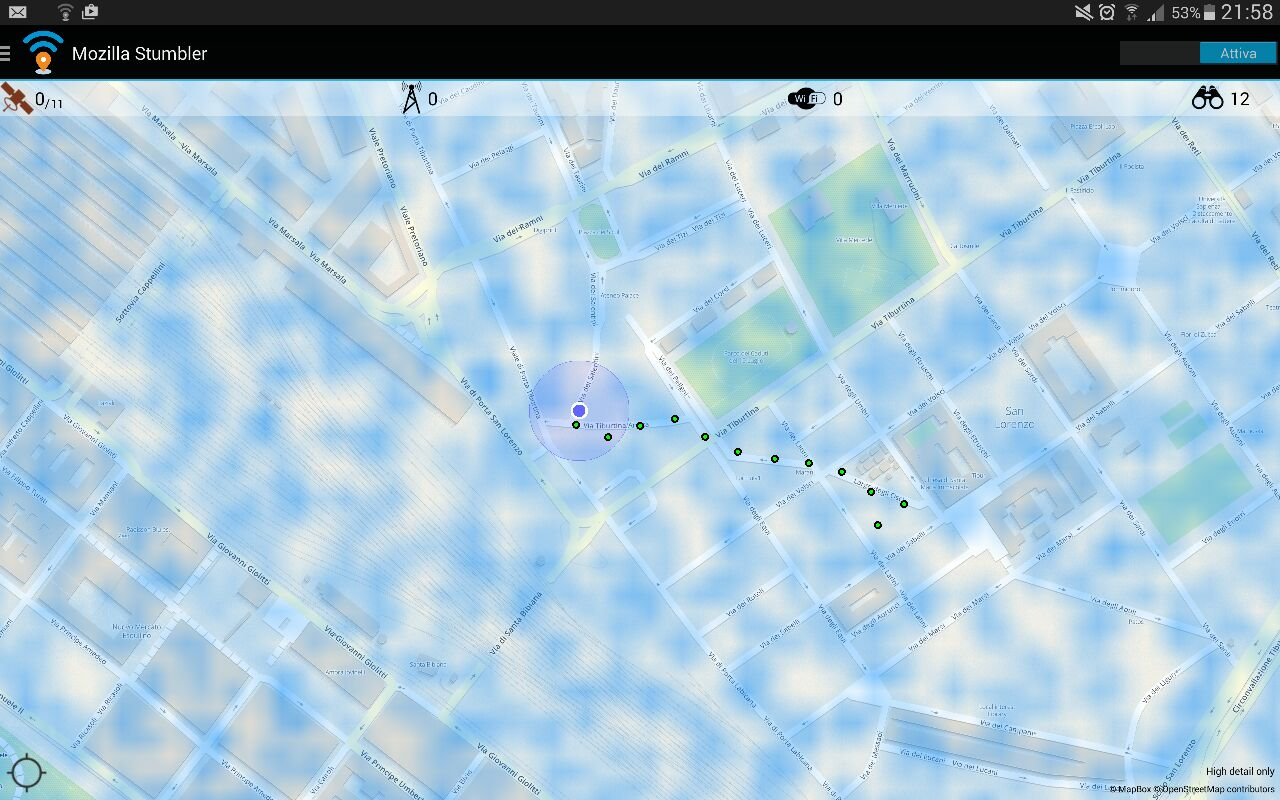
\includegraphics[width=0.8\textwidth]{./Immagini/Dati/appmap.jpg}
	\caption{\emph{Screen} dell'applicazione attiva}
	\label{fig:mapp}
\end{figure}
Il progetto è ormai maturo e, come si può osservare nelle mappe in fig. \ref{fig:mapp} e \ref{fig:wapp} la copertura del mondo è molto capillare.
\begin{itemize}
 \item La prima mostra un esempio di utilizzo del programma a San Lorenzo, nel percorso tra le nostre due abitazioni. I pallini verdi sono i punti GPS delle rilevazioni complete (WiFi + rete cellulare) effettuate durante il tragitto. Come si può notare sono piuttosto fitti: 4 0 5 per ogni isolato. Le aree sfumate in blu mostrano invece, in maniera approssimata per motivi di privacy, l'esito dell'eleborazione di tutte le precedenti osservazoni nell'area, ovvero tutti i router WiFi e le antenne ricostruiti fin ora. La mappa è fittissima, ma questo non deve trarre in inganno: è ancora incompleta e per certi versi inaffidabile. Un esempio diretto sono le numerose ricostruzioni che appaiono in mezzo ai binari della stazione Termini: quelle derivano dai WiFi all'interno dei treni a cui si collegano i viaggiatori, ma che essendo oggetti in moto non possono essere usati ai fini della geolocalizzazione e pertanto dovrebbero essere filtrati ed esclusi dal database.
  \item La seconda mappa mostra invece la copertura globale raggiunta dal progetto. Sebbene risulti uno stadio abbastanza avanzato, si può notare come ci siano ancora delle disparità di mappatura anche tra gli stati ad alta presenza tecnologica: si confrontino ad esempio le capitali della Cina e del Giappone. Inoltre, essendo un progetto collaborativo open source e con sede negli Stati Uniti, sì può vedere come gli stati in cui la cultura open è meno diffusa o quelli in tensione con gli USA per quanto riguarda la politica estera risultino globalmente meno mappati. Un esempio emblematico potrebbe essere la differenza tra Nord Korea e Sud Korea.
\end{itemize}

\begin{figure}[b!]
	\centering
	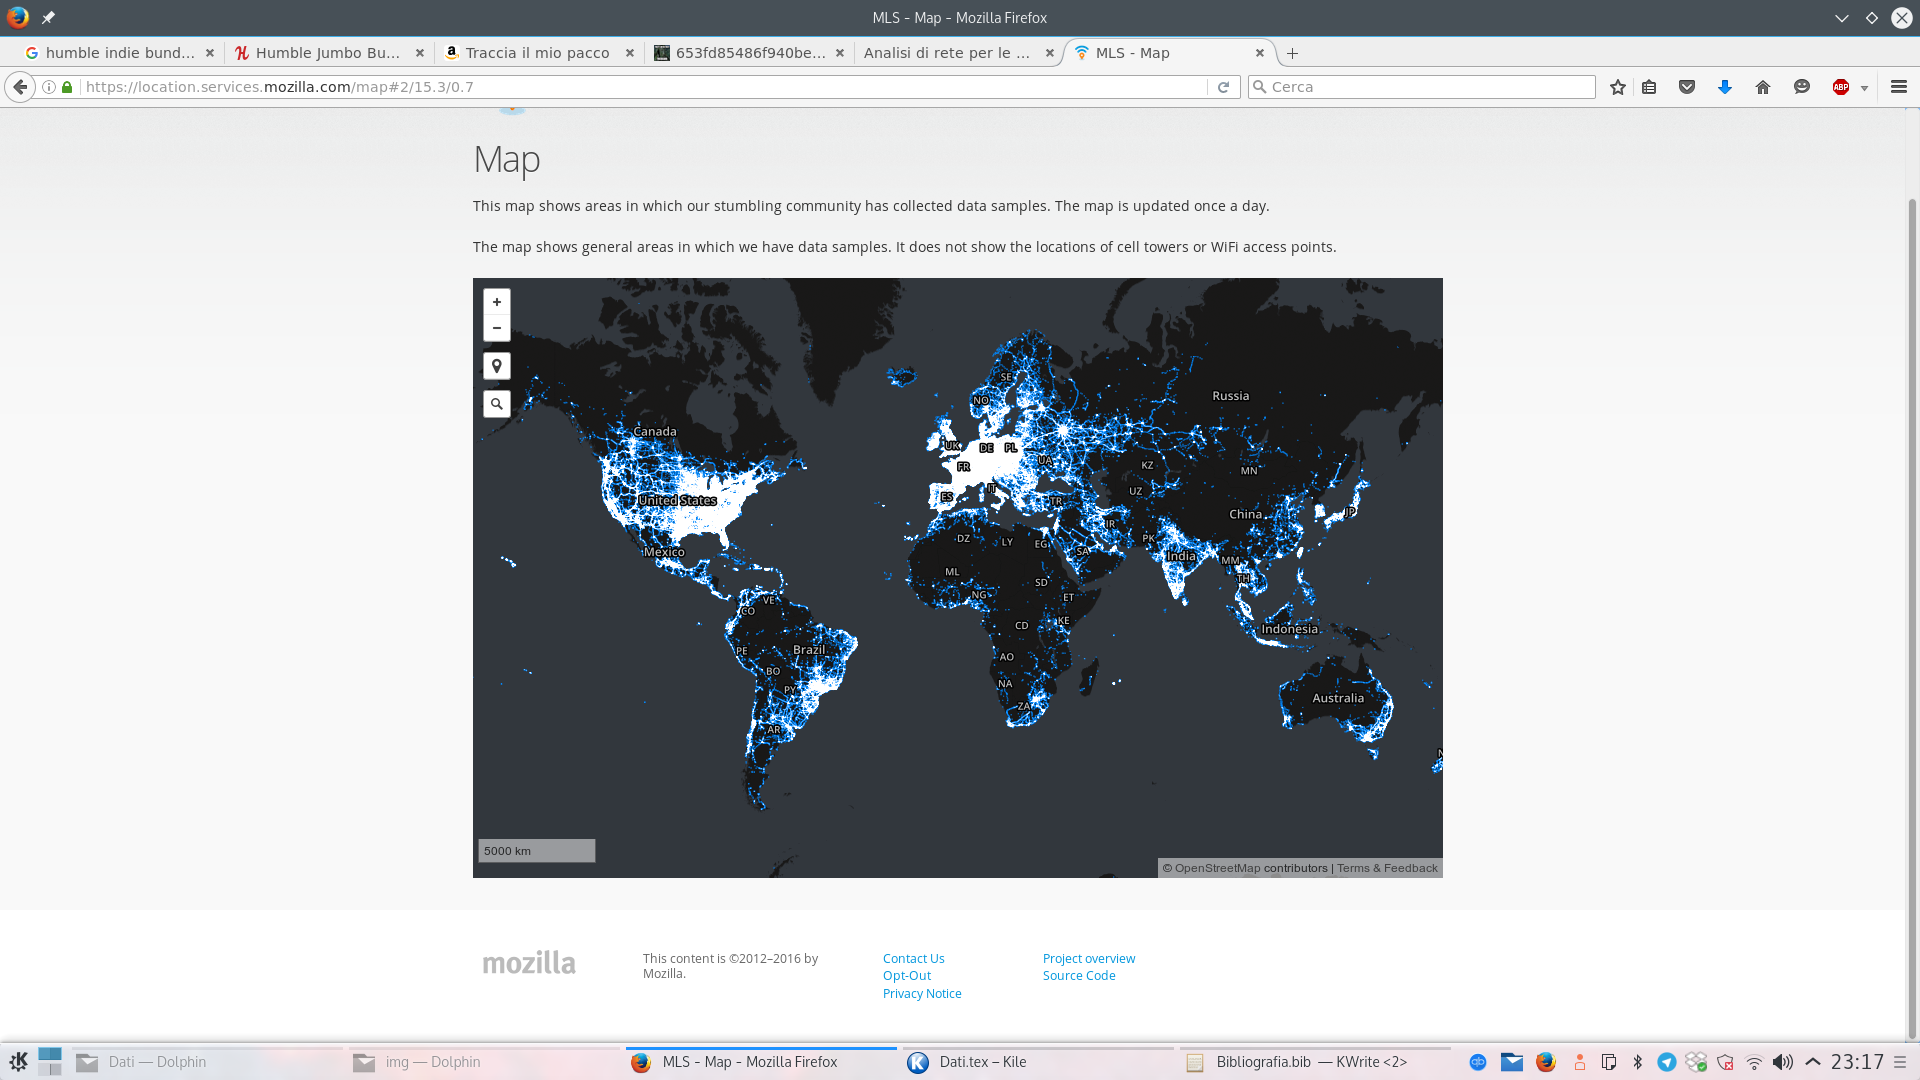
\includegraphics[width=0.8\textwidth]{./Immagini/Dati/MLSmap.png}
	\caption{Immagine della mappa fornita da Mozilla}
	\label{fig:wapp}
\end{figure}

Dato l'approccio di \emph{crouwdsourcing} collaborativo, i dati sono tanti e la copertura mondiale, continuamente aggiornati, aperti, facilmente scaricabili in database ordinati, puliti e ben documentati. Di seguito sono elencate alcune statistiche per avere un'idea dei numeri in gioco:
\begin{table}[t]
\centering
\caption{Alcune statistiche dei dati forniti da MLS}
\parbox{0.45\textwidth}{
\centering
	\begin{tabular}{cc}
	\toprule
	data 				&total\\
	\midrule
	Wifi Networks 			&521.610.000\\
	Wifi Observations 		&1.1006.560.000\\
	MLS Cells 			&20.390.000\\
	MLS Cell Observations 	&2.468.460.000\\
	OpenCellID Cells 		&7.990.000\\
	\midrule
	\end{tabular}
\label{tab:statacq}
}
\\
\parbox{0.45\textwidth}{
\centering
	\begin{tabular}{ccc}
	network 		&Italy 		&United States\\
	\midrule
	GSM (2G) 		&132.468 		&230.236\\
	UMTS (3G) 	&516.379 		&976.603\\
	LTE (4G) 		&96.489 		&1.595.402\\
	Total Cells 	&745.336 		&2.802.241\\
	WiFis 		&9.844.682 	&175.599.375\\
	\bottomrule
	\end{tabular}
\label{tab:statreg}
}
\label{tab:expectedfluoZnSe}
\end{table}

Mozilla Location Service funziona sia con le antenne cellulari che con i WiFi, soltanto che attulamente i dati della mappa WiFi (mostrati approssimati nella mappa precedente) non possono essere resi pubblici per questioni relative alle norme sulla privacy vigenti sia negli Stati Uniti sia in altre nazioni.

Pertanto gli unici dati attualmente liberamente disponibili (dominio pubblico, licenza CC0) sono quelli sulle antenne radio delle varie generazioni: 2G (GSM), 3G (UMTS), 4G (LTE).
I dati forniti da Mozilla sono un'estensione di quelli già disponibili sulla piattaforma \citetitle{cellid}, anche loro open (licenza CC-BY-SA 3.0).

Questi sono dunque i dati che abbiamo analizzato in questa nostra tesina.

\clearpage
\section{MLS dataset}
\label{sec:mls}
I dati scaricabili dal sito del progetto Mozilla Location Service appaiono come in tabella \ref{tab:esempiodati}

I dati vengono forniti in un file CSV, le cui voci, secondo la documentazione ufficiale, sono organizzate nella seguente maniera:

\begin{description}
 \item[radio] Network type. One of the strings GSM, UMTS or LTE.
 \item[mcc] Mobile Country Code. An integer, for example 505, the code for Australia.
 \item[net] For GSM, UMTS and LTE networks, this is the mobile network code (MNC). An integer, for example 4, the MNC used by Vodaphone in the Netherlands.
 \item[area] For GSM and UMTS networks, this is the location area code (LAC). For LTE networks, this is the tracking area code (TAC). An integer, for example 2035.
 \item[cell] For GSM and LTE networks, this is the cell id or cell identity (CID). For UMTS networks this is the UTRAN cell id, which is the concatenation of 2 bytes of radio network controller (RNC) code and 2 bytes of cell id. An integer, for example 32345.
 \item[unit] For UMTS networks, this is the primary scrambling code (PSC). For LTE networks, this is the physical cell id (PCI). For GSM networks, this is empty. An integer, for example 312.
 \item[lon] Longitude in degrees between -180.0 and 180.0 using the WSG 84 reference system. A floating point number, for example 52.3456789.
 \item[lat] Latitude in degrees between -90.0 and 90.0 using the WSG 84 reference system. A floating point number, for example -10.034.
 \item[range] Estimate of radio range, in meters. This is an estimate on how large each cell area is, as a radius around the estimated position and is based on the observations or a knowledgeable source. An integer, for example 2500.
 \item[samples] Total number of observations used to calculate the estimated position, range and averageSignal. An integer, for example 1200.
 \item[changeable] Whether or not this cell is a position estimate based on observations, and therefore subject to change in the future, or is an exact location entered from a knowledgeable source. A boolean value, encoded as either 1 (for “changeable”) or 0 (for “exact”).
 \item[created] Timestamp of the time when this record was first created. An integer, counting seconds since the UTC Unix Epoch of 1970-01-01T00:00:00Z. For example, 1406204196, which is the timestamp for 2014-07-24T12:16:36Z.
 \item[updated] Timestamp of the time when this record was most recently modified. An integer, counting seconds since the UTC Unix Epoch of 1970-01-01T00:00:00Z. For example, 1406204196, which is the timestamp for 2014-07-24T12:16:36Z.
 \item[averageSignal] Average signal strength from all observations for the cell network. An integer value, in dBm. For example, -72.\\
 This field is only used by the OpenCellID project and historically has been used as a hint towards the quality of the position estimate.
\end{description}

I dati forniti sono di tipo aggregato, ovvero riportano il numero di osservazioni per antenna ed il risultato della stima della sua posizione. Esistono anche dati grezzi, ovvero corrispondenti alle singole osservazioni dei singoli utenti. Tale dataset però non viene reso pubblicamente disponibile, in quanto contenente diverse informazioni, anche di carattere dinamico, utili a tracciare il singolo individuo. È allo studio un meccanismo di autorizzazioni per permettere agni utenti consci degli eventuali rischi di pubblicare i dati che li riguardano.

I valori di latitudine e longitudine per le coordinate nelle proiezioni geografiche seguono il sistema di riferimento dettato dalla convenzione WSG 84 Web Mercator.
\begin{table}[ht!]
\centering
\caption{Esempio del dataframe MLS}
	\begin{tabular}{ccccccc}
	\toprule
radio 	&mcc 	&net &area 	&cell \\	
GSM 		&262 	&7 	&20205 	&2227 \\	
GSM 		&262 	&2 	&685		&6132 \\	
GSM 		&262 	&1 	&14660 	&39399 \\	
GSM 		&262 	&7 	&20202 	&33063 \\
GSM 		&262 	&7 	&20205 	&2472 \\
\midrule
unit 		 &lon	&lat 		&range 	&samples \\
NaN		&13.308816 	&52.512122	&147481 	&14586 \\
NaN		&7.018766 	&49.223543	&14976 	&5336 \\
NaN		&9.879624 	&51.335388	&101430 	&4049 \\	
NaN		&13.327494	&52.516999	&148854 	&6412 \\	
NaN		&13.296922	&52.507817	&132401 	&11216 \\	
\midrule
changeable 	&created 		&updated 		&averageSignal\\
1 			&1299573448 	&1453335612 	&-64\\
1 			&1299584114 	&1453337312 	&-74\\
1 			&1299693112 	&1453335486 	&-57\\
1 			&1301668631 	&1453335612 	&-61\\
1 			&1301668631 	&1453335612 	&-65\\
\bottomrule
	\end{tabular}
\label{tab:esempiodati}
\end{table}

\subsection{Data selection}
Una volta scaricati i dati aggregati dalla pagina web \lstinline{https://location.services.mozilla.com/downloads} sono cominciate le operazioni di selezione dei dati. Il data sample riguarda tutti i continenti e risulta molto grosso (un file csv di circa 650 MB), per cui è necessario ridurlo il più possibile per poterlo maneggiare con il nostro limitato quantitativo di RAM.

Una prima grossolana ma efficiente scrematura riguarda i dati caratterizzati da un mobile county code non italiano, si è pertanto imposta la condizione
\begin{lstlisting}
mcc == 222
\end{lstlisting}
Successivamente vengono scartati i dati ritenuti inaffidabili, ovvero con soltanto una rivelazione da parte degli utenti
\begin{lstlisting}
samples > 1
\end{lstlisting}

Adesso che il datasample si è ridotto molto possiamo effettuare delle operazioni computazionalmente un po' più pesanti: vogliamo eliminare tutte le rilevazioni al di fuori del Grande Raccordo Anulare, che per semplicità è stato schematizzato come una circonferenza di raggio 10 km con centro esattamente nol Colosseo. Per far questo serve definire una nozione di distanza. Dato che i nostri sono dati geolocalizzati sarebbe naturale introdurre una distanza geodesica. A tal fine abbiamo usato la libreria \emph{geopy}, che contiene due definizioni differenti:

\begin{itemize}
 \item Great circle distance: la distanza geodesica su una sfera. Per due punti non agli antipodi passa sempre una circonferenza di raggio massimo lungo cui scorre la geodesica, ovvero il cammino di minima distanza. 
 \item Vincenty distance: la distanza geodesica su un ellissoide oblato. Tale distanza tiene in conto che la Terra non è una sfera perfetta ma è invece leggermente schiacciata ai poli. Delle due è quella più accurata, ma anche quella più difficile da calcolare numericamente.
\end{itemize}
L'ulteriore condizione da soddisfare per i dati risulta dunque
\begin{lstlisting}
geodesicDistance(place) <= raggioRaccordoAnulare
\end{lstlisting}

Si sono fatte differenti prove sia con \lstinline{vincenty} (più lenta) che con \lstinline{great_circle} (leggermente più veloce), ma i tempi di calcolo risultavano comunque spropositati. Pertanto abbiamo fatto una approssimazione: dato che la città di Roma sottende un angolo solido minuscolo rispetto alla totalità del pianeta, abbiamo ritenuto accettabile usare una distanza euclidea, ovviamente trasformando in metri le coordinate angolari di latitudine e longitudine con i relativi fattori di scala, dettati dal raggio terrestre.

La distanza euclidea coinvolge solo quadrati è radici quadrate, risultando nel complesso circa dieci volte più veloce delle altre due concorrenti. Il prezzo da pagare è una leggerissima imprecisione, del tutto trascurabile alle nostre scale. La funzione utilizzata è pertanto
\begin{lstlisting}
def euclideanDistace(x,y):
    return numpy.sqrt(numpy.square(x) + numpy.square(y))
\end{lstlisting}
Da notare il fatto che per il calcolo algebrico è stata utilizzata la libreria \emph{numpy} invece che la libreria \emph{math} built-in in Python, poiché è più veloce (è scritta in C) e supporta le operazioni direttamente su vettori di coordinate.

I dati sono stati importati in un dataframe tabulare usando la libreria \emph{pandas}. Questo che ci ha permesso di effettuare facilmente tutte le \emph{query} necessarie per il filtraggio dei dati.
\clearpage
\begin{table}[t]
\caption{Esempio del dataframe da noi utilizzato}
	\begin{tabular}{ccccccccc}
	\toprule
radio	&net &cell 	&lon 	 &lat 		&range 	&samples 	&distance &degree\\
GSM		&10 	&29369 	&12.630353 &41.892274 	&10568 	&2 		&11457 	&2412\\
GSM 		&10 	&28691 	&12.620040 &41.890106 	&9674 	&2 		&10598 	&2361\\
GSM 		&88 	&19451 	&12.531354 &41.986043 	&2172 	&4 		&11129 	&179\\
GSM 		&88 	&16608 	&12.605920 &41.918988 	&4129 	&7 		&9953 	&621\\
GSM 		&88 	&55647 	&12.604219 &41.928254 	&9245 	&23 		&10201 	&2048\\
\bottomrule
	\end{tabular}
\label{tab:datinostri}
\end{table}

A questo punto abbiamo finalmente il nostro datasample della città di Roma: circa 7000 antenne in un file csv agevolmente maneggiabile di circa 1MB.

\begin{figure}[b!]
	\centering
	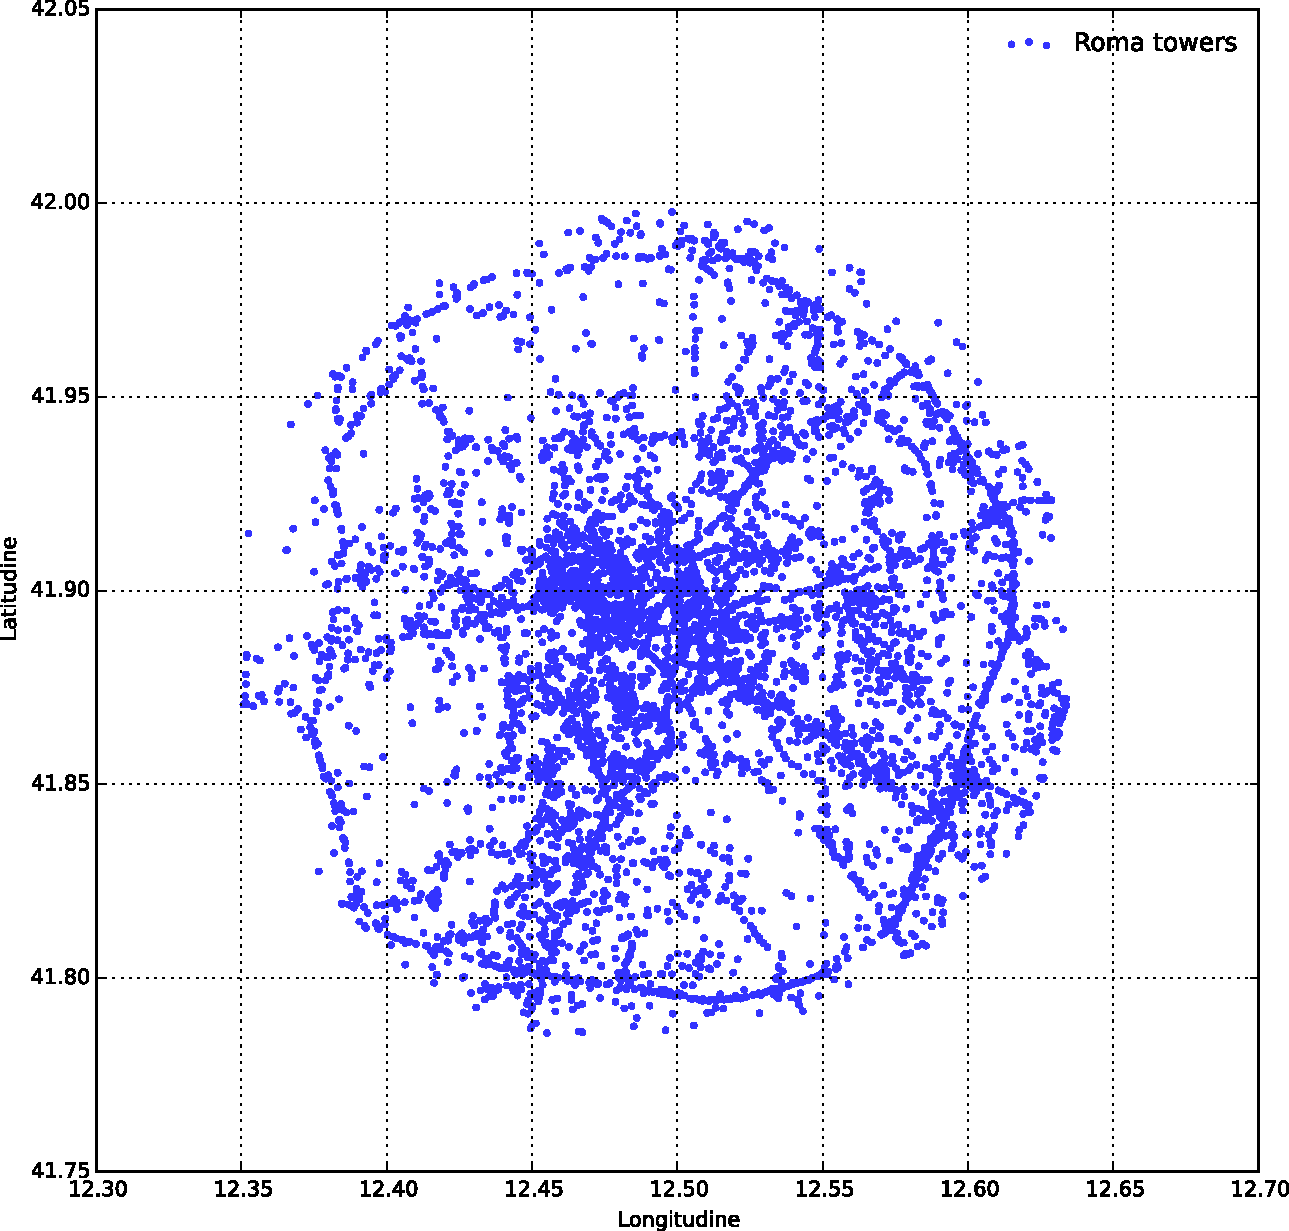
\includegraphics[width=0.5\textwidth]{./Immagini/Dati/roma}
	\caption{Scatterplot non georeferenziato delle antenne di Roma.}
	\label{fig:napp}
\end{figure}

Per visualizzare agevolmente i nostri dati serve una mappa georeferenziata, preferibilmente interattiva. A tal fine per il notebook di IPython abbiamo usato la libreria \emph{gmaps}, che dà semplice accesso inline alle mappe di Google Maps dando la possibilità di creare una \emph{heatmap}, mentre per l'HTML di questa presentazione abbiamo usato le analoghe funzioni della libreria \emph{gmplot}:

\begin{lstlisting}
roma = pandas.read_csv("../data/Roma_towers.csv")
coordinate = roma[['lat', 'lon']].values
heatmap = gmaps.heatmap(coordinate)
gmaps.display(heatmap)

colosseo = (41.890183, 12.492369)
mappa = gmplot.GoogleMapPlotter(41.890183, 12.492369, 12)
mappa.heatmap(roma.lat.values,roma.lon.values)
mappa.draw("../doc/heatmap.html")
\end{lstlisting}
(per scrivere queste poche linee di codice c'è voluto un intero pomeriggio!)

\begin{figure}[ht!]
	\centering
	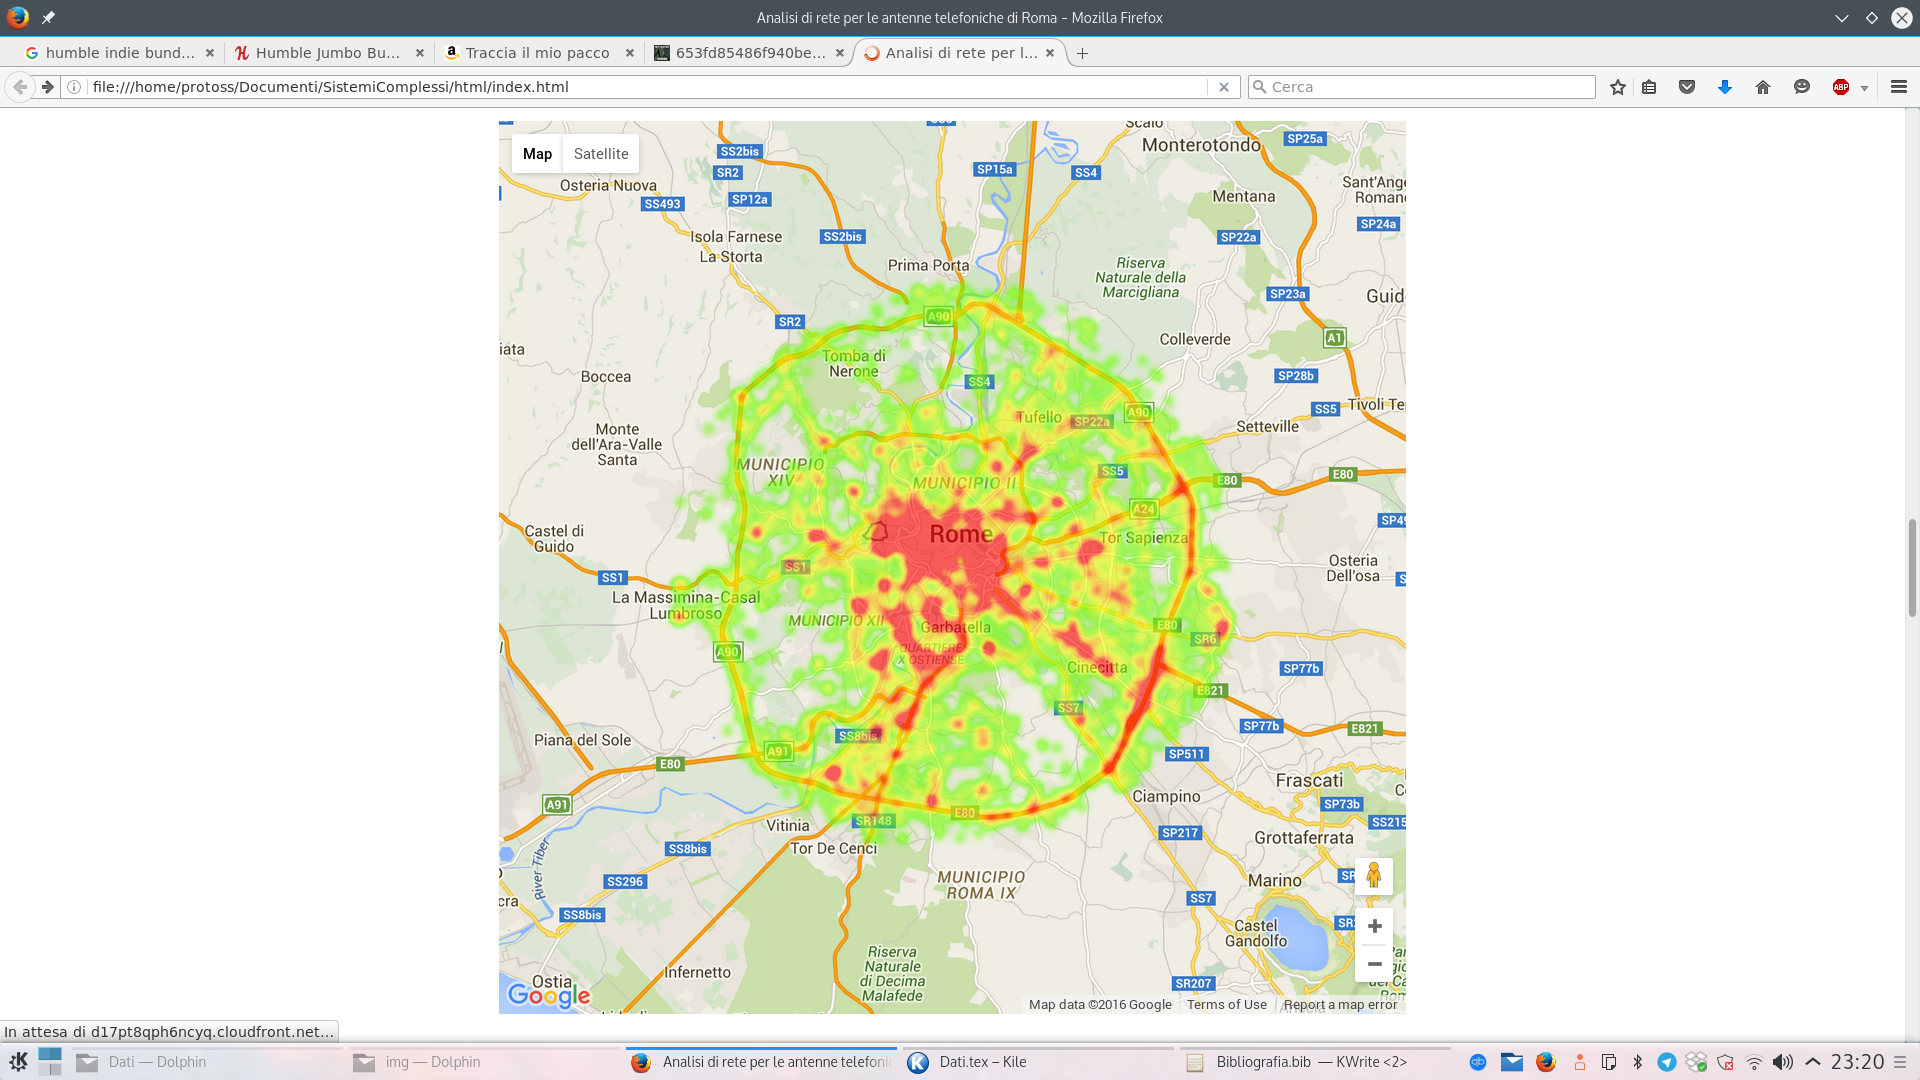
\includegraphics[width=0.5\textwidth]{./Immagini/Dati/Ourmap.png}
	\caption{Heatmap delle antenne telefoniche di Roma}
	\label{fig:happ}
\end{figure}

% \clearpage
\subsection{Analisi del raggio di copertura delle antenne}
Dato che ci servirà fare grafici con scale logaritmiche eliminiamo i dati di antenne che presentano un raggio nullo

\begin{lstlisting}
range =! 0
\end{lstlisting}

Il raggio minimo risulta essere 1m, mentre quello massimo 20341m. Dato che il raggio del Grande Raccordo Anulare è circa 10km questo significa che ci saranno antenne con un grado di connessione totale.
% TODO forse spostare questa considerazione a quando si è spiegato il criterio di linking. TODO spiegare la possibile casa di questi valori di raggi così bassi
Facciamo un istogramma log-log per la distribusione del raggio di copertura, sia con la canalizzazione lineare sugli interi, sia con una canalizzazione logaritmica in base 2, per ridurre il rumore sulla coda.

\begin{figure}[b!]
	\centering
	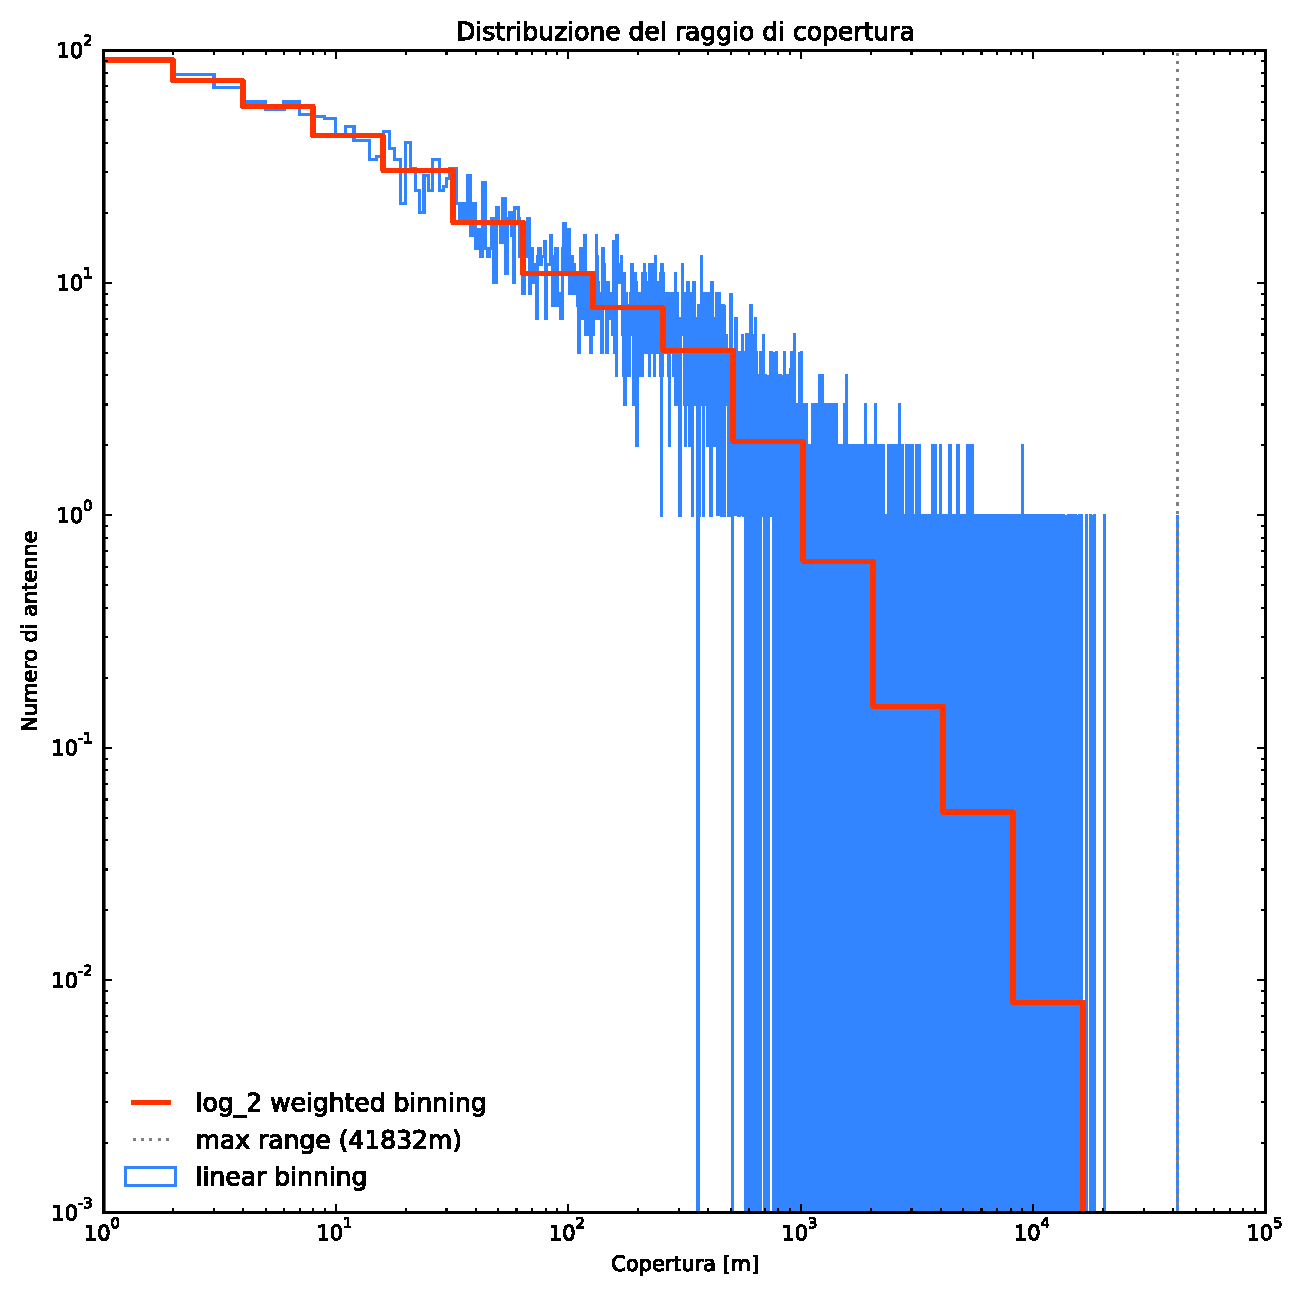
\includegraphics[width=0.5\textwidth]{./Immagini/Dati/logbin}
	\caption{Istogramma log-log dei raggi con log-binning.}
	\label{fig:lograggi}
\end{figure}

La canalizzazione logaritmica pesata permette di osservare l'andamento ben sotto il singolo conteggio, ampliando di una decade l'intervallo di osservazione.

In figura \ref{fig:lograggi} si può vedere come l'andamento sia abbastanza power-law su diverse decadi, soprattutto fino a \lstinline{conteggio = 1}. Per verificare ulteriormente questo fatto abbiamo generato anche la curva del frequency-rank (Figura \ref{fig:rfreqrank}), che risulta seguire senza esitazioni il trend delineato dagli istogrammi.
%TODO cercare di spiegare questa plaw
Il frequency-rank si ottiene ordinando in maniera decrescente il numero di conteggi per ogni canale unitario e associando un relativo ranking intero decrescente ai raggi corrispondenti. 

\begin{figure}[t]
	\centering
	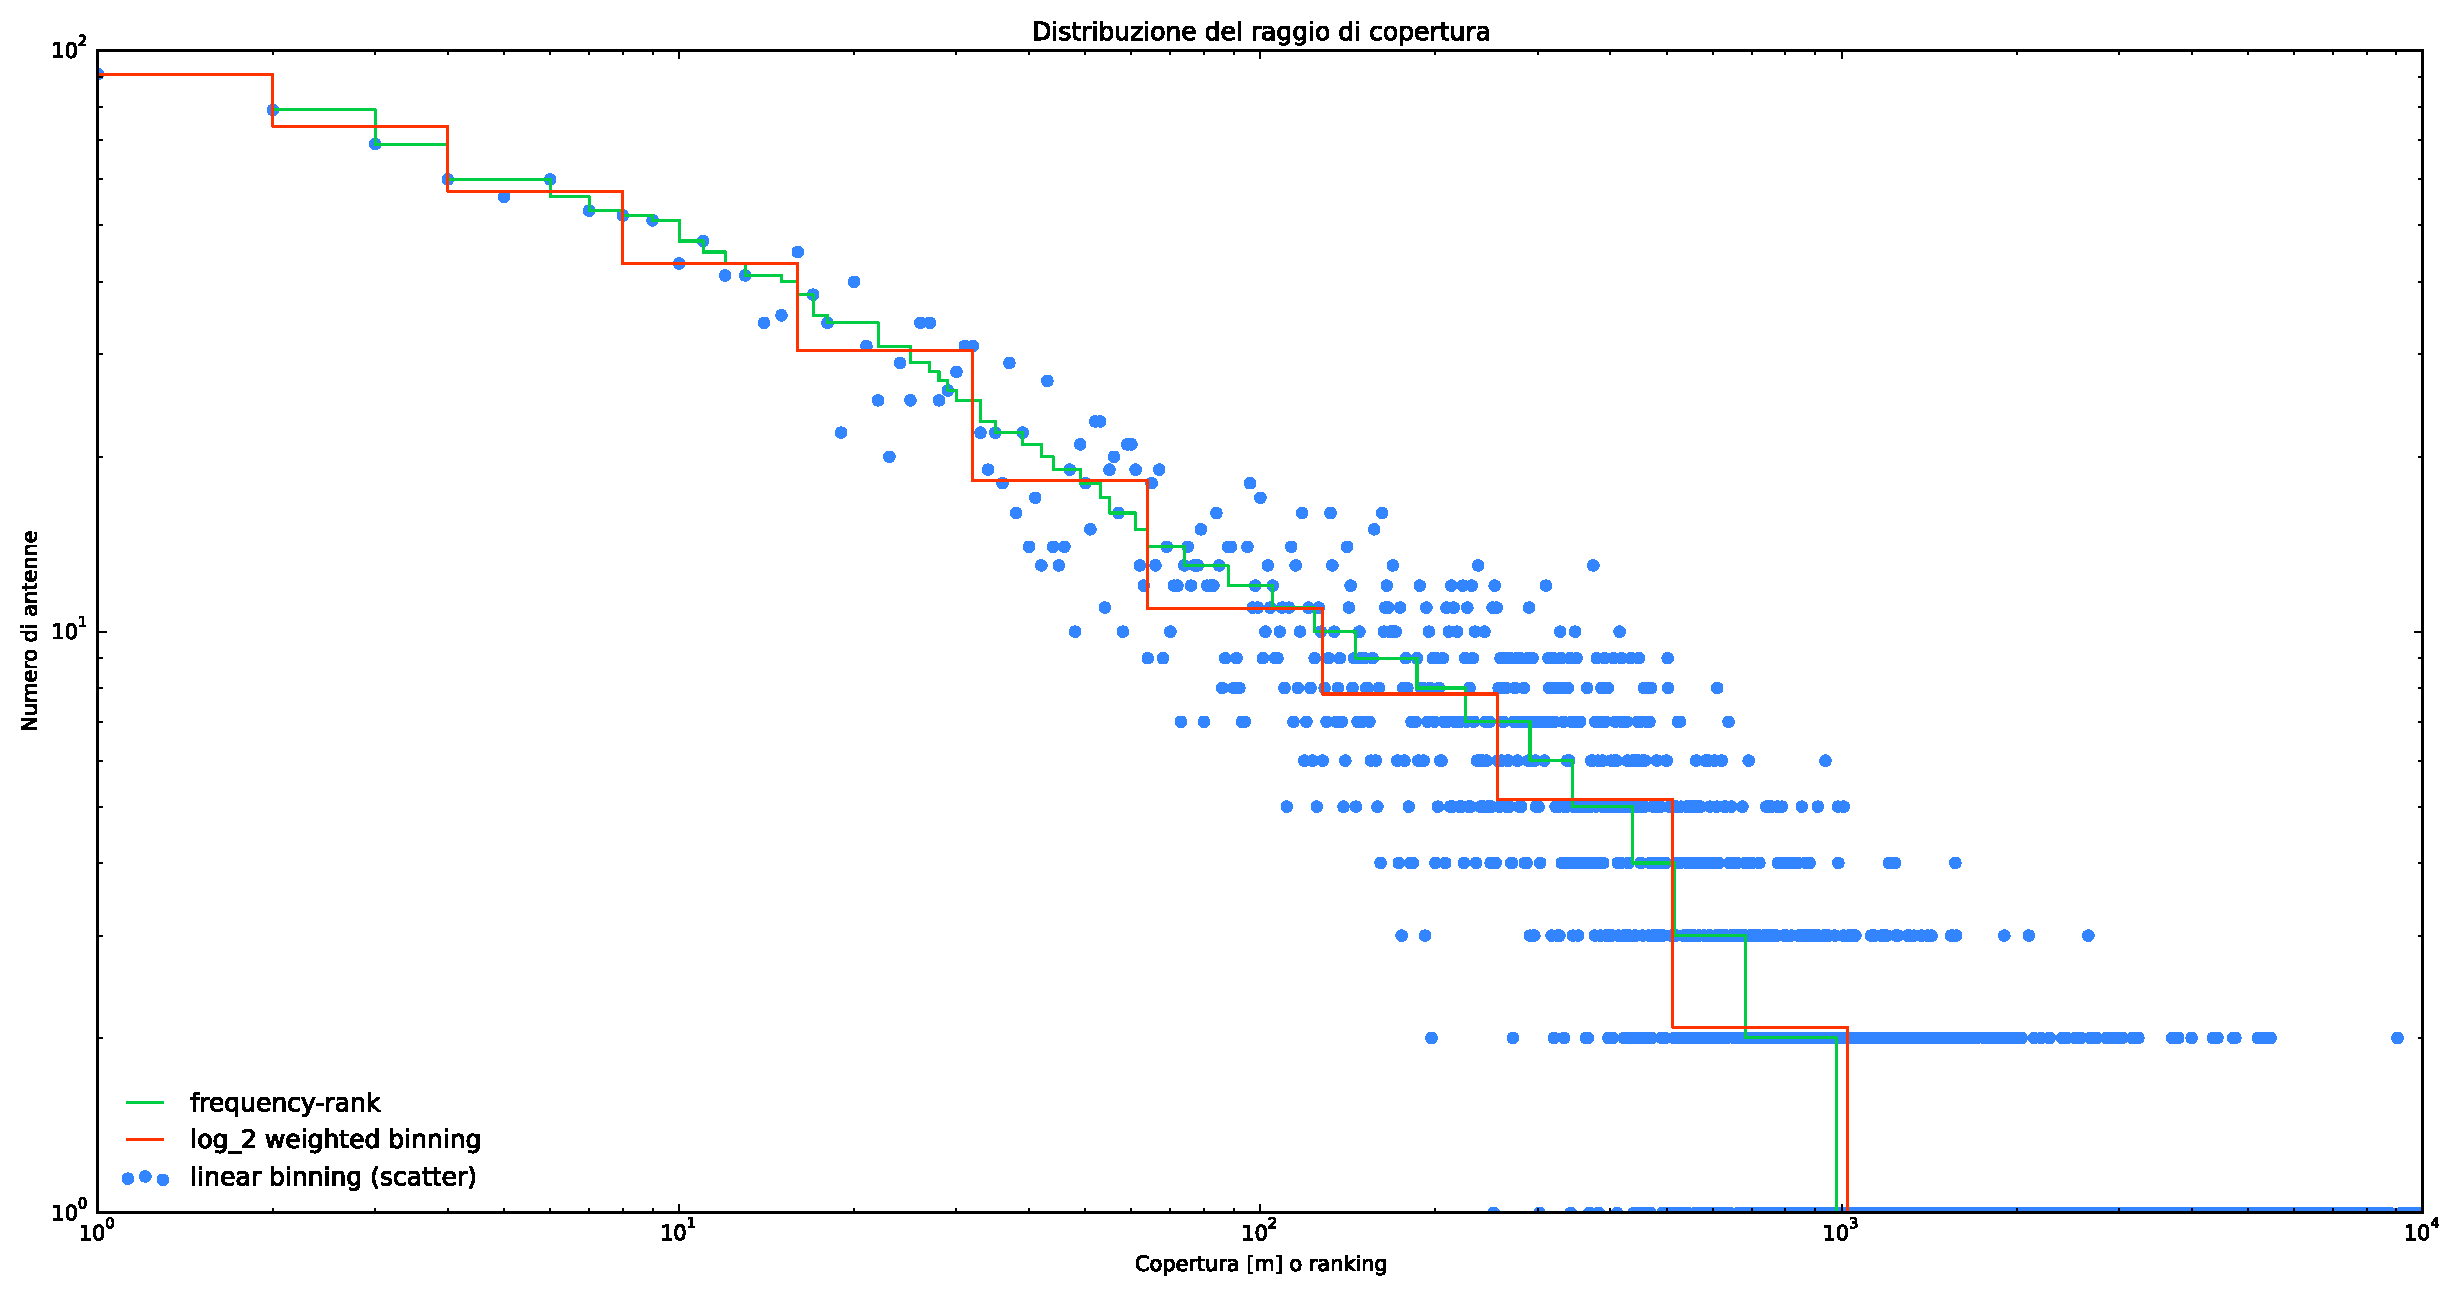
\includegraphics[width=0.8\textwidth]{./Immagini/Dati/rangefreqrank}
	\caption{Frequency rank dei raggi in scala log-log}
	\label{fig:rfreqrank}
\end{figure}

% Si è infine analizzata la distribuzione cumulata, lasciata nel grafico seguente non normalizzata. La distribuzione cumulata $C(x)$ rappresenta la probabilità che la variabile random assuma un valore minore o uguale a $x$.

% \begin{figure}[ht!]
% 	\centering
% 	\includegraphics[width=0.5\textwidth]{./Immagini/Dati/cumulata}
% 	\caption{Frequency rank dei raggi in scala log-log}
% 	\label{fig:rfreqrank}
% \end{figure}
% !TEX encoding = UTF-8
% !TEX TS-program = pdflatex
% !TEX root = ../Relazione.tex
% !TEX spellcheck = it-IT
\clearpage
%%%%%%%%%%%%%%%%%%%%%%%
\section{Network breakdown}
\label{sec:attaack}
%%%%%%%%%%%%%%%%%%%%%%%
%(formerly "Analisi percolativa" ma questo è un titolo noioso, meglio una roba più deep impact ogliea) 

Una volta osservate le distribuzioni del grado nelle reti delle quattro compagnie e nella rete complessiva formata da tutte le antenne comprese nell'area metropolitana di Roma, procediamo con lo studio percolativo. Si è scelto di simulare due differenti scenari in cui i nodi della rete vengono disabilitati \textcite{Barbalbert2000}. Nel primo scenario si è ipotizzato un attacco intenzionale che cominciasse dai nodi con maggior grado, nel secondo una rimozione random.

Lo scopo è studiare l'andamento, in funzione della percentuale di nodi rimossi, del diametro $D$ della rete e della dimensione del cluster più grande (verificando che esso sia il Giant Cluster della rete) rapportata al numero totale di nodi sopravvissuti. A seconda di come la rete si comporterà, sarà possibile dedurne la robustezza nei due scenari, in modo tale da poter confrontare meglio tale comportamento con quello di una rete scale-free o random di pari grado medio $\langle k \rangle$.

In tutti e cinque i campioni di rete che abbiamo analizzato, sono stati conteggiati gli andamenti di alcune grandezze topologiche e statistiche di interesse: oltre a dimensione del giant cluster, $D$, anche $\langle l \rangle$, coefficiente di clustering globale $C$, $\langle k \rangle$ e $\langle k^2 \rangle/\langle k \rangle$. I grafici ottenuti sono stati messi a confronto a quelli ottenuti con le reti generate secondo i modelli.

È importante ricordare che la rete reale ha ovviamente delle contromisure per evitare la caduta delle comunicazioni. Le antenne trasmettono segnali tra loro su due bande di frequenza: una \emph{user-side}, dedicata alle normali trasmissioni tra utenti del servizio, e una dedicata a un complesso sistema di feedback gestito da degli \emph{hub}(grosse antenne con raggio sui $20\:km$). Questa struttura gerarchica permette, nel caso di caduta di una antenna o di un improvviso eccessivo carico in una zona circoscritta, che gli hub gestiscano potenza e capacità delle antenne circostanti mentre vengono inviati tecnici per un intervento sul luogo.

Questo sistema ha un certo tempo di reazione. L'analisi da noi svolta pertanto suppone che la caduta della rete avvenga in un tempo inferiore, in una sorta di approssimazione adiabatica. Inoltre, la sola caduta degli hub sarebbe già sufficiente a compromettere seriamente l'integrità della rete (le antenne avrebbero difficoltà a coordinare le comunicazioni tra loro), ma nella nostra ipotesi di mesh-network distribuita ci interessano soltanto le comunicazioni nelle frequenze user-side. Usando questo modello semplificato siamo riusciti a ottenere alcune informazioni su una ipotetica rete cittadina di questa natura.

\subsection{Speedup del codice (parte 1: multiprocessing)}

Per le simulazioni di attacco intenzionale e random failure sulle reti in esame e lo studio approfondito dell'andamento delle grandezze statistiche e topologiche durante l'analisi percolativa, abbiamo inizialmente utilizzato \emph{networkx}, una libreria di Python piuttosto completa dedicata alle reti.

Tuttavia questa si è rivelata una scelta sbagliata, in quanto networkx, pur essendo molto completa e semplice da usare, non è particolarmente ottimizzata dal punto di vista dell'efficienza di calcolo. Questo perché è interamentente scritta in Python, anche per le sue routine più interne e non implementa alcun tipo di parallelismo built-in.

Creare, manipolare e disegnare i grafi sono operazioni semplici e immediate, ma ma quando si cercano di usare le funzioni più pesanti dal punto di vista del calcolo, come per esempio quella per determinare il diametro della rete, networkx appare del tutto non soddisfacente.

Per esempio, il calcolo di diametro, average path lenght, coefficiente di clustering e dimensioni del giant cluster impiegava 20 secondi per una singola iterazione con la rete Tre (la più piccola, circa 1400 nodi), 50 secondi per Tim e Vodafone (circa 1800 nodi entrambe) mentre con la rete Wind (la più grande, con circa 2350 nodi) impiegava ben 2.5 minuti. Questo dato, moltiplicato per i 100 passi richiesti, porta ad una previsione di più di 6 ore di calcolo per l'analisi percolativa di tutte le singole reti.

Abbiamo osservato che i tempi scalano all'incirca quadraticamente con il numero di nodi, per cui per lo studio della rete complessiva di tutta Roma sarebbero richiesti 20 minuti per una iterazione e quasi 30 ore di calcolo per l'analisi completa. Queste considerazioni rendevano di fatto impraticabile questa strada.

\begin{figure}[ht!]
	\centering
	
\includegraphics[width=0.55\textwidth]{./Immagini/Attack/meme_Leonida.jpg}
\end{figure}

Dato che i tempi di calcolo richiesti per l'analisi percolativa risultavano spropositati, soprattutto nel caso di random failure, abbiamo cercato dei modi per velocizzare il calcolo ed aggirare il problema.

In primis si è cercato di evitare operazioni cicliche sui vettori dinamici, come \lstinline{pop()} e \lstinline{append()} e di utilizzare sempre librerie python ottimizzate e internamente scritte in C, come ad esempio \emph{numpy}. Già questo permette operazioni su grossi vettori con un incremento di prestazioni rispetto al python puro di almeno il doppio.

Inoltre si è tentato di sfruttare i diversi core della macchina, facendo degli esperimenti di rudimentale calcolo parallelo. In pratica si è cercato di rendere il codice non sequenziale, in modo da usare funzioni del tutto indipendenti e poter scrivere tutto quanto in termini di funzioni \lstinline{map()} per poi utilizzare la libreria built-in \emph{multiprocessing} e fare una prima parallelizzazione. 

\begin{lstlisting}
import multiprocessing
cpus = multiprocessing.cpu_count()
pool = multiprocessing.Pool(processes=cpus)
pool.map(function, array)
\end{lstlisting}

Abbandonare il paradigma sequenziale rendendo le funzioni totalmente indipendenti tra loro fa sì che esse possano girare in contemporarea riducendo il tempo di calcolo, ma nel contempo aumenta il quantitativo di RAM richiesta dal programma, quasi dello stesso fattore. Pertanto bisogna fare attenzione a far girare il programma su una macchina adeguata sotto tutti i punti di vista.

Purtroppo peò nel nostro caso questo approccio non si è rivelato adatto. Nel fare i tentativi vedevamo che i processori lavoravano insieme al 100\% per un primo periodo, per poi ibernarsi in una eterna fase di stallo al 20\% del carico, probabilmente per incongruenze nel messaging tra le varie istanze di python. Non possedendo sufficienti conoscenze su calcolo parallelo e cloud computing per poter risolvere velocemente il problema, abbiamo dunque abbandonato questo aproccio.

\begin{figure}[h!]
	\centering
	
\includegraphics[width=0.55\textwidth]{./Immagini/Attack/meme_Boromir.jpg}
\end{figure}

\subsection{Strategie di attacco}
\label{subsec:atakstrat}
L'esigenza di provare a parallelizzare il codice ci ha portato a due versioni differenti della funzione di attacco intenzionale: una sequenziale e una parallela. Entrambe le varianti rimuovono circa l'1\% dei nodi per volta: 

\begin{itemize}
 \item La funzione sequenziale elimina l'insieme dell'1\% dei nodi più importanti, analizza la rete e calcola il prossimo insieme di 1\% di nodi da rimuove.
 \item La funzione parallela ha invece un comportamento più adiabatico: guarda il grafo iniziale e fa una classifica assoluta dei nodi per importanza, rimuovendone di volta in volta l'1\% in maniera ordinata.
\end{itemize}

Possiamo supporre che un reale attacco alla rete sia portato avanti con modalità adiabatiche: un ipotetico terrorista piazza nella notte delle cariche esplosive sotto le antenne che ritiene fondamentali e poi le fa scoppiare in un secondo momento tutte in una volta. A titolo di esempio, possiamo immaginare che l'attacco si consideri riuscito quando metà dell'area metropolitana rimane isolata senza possibilità di comunicare. Questo è il parametro finale in base al quale viene scelta la sequenza di antenne da far esplodere.

Ma chi garantisce che questa sequenza coincide con gli N nodi di grado maggior all'istante iniziale? In altre parole: è questa una strategia \emph{ottimale}?\\
La risposta è no! La strategia ottimale è quella che, a parità di risultato, coinvolge il minor numero di antenne fatte eplodere, anche per minimizzare il rischio di essere scoperto nella notte mentre piazza l'esplosivo in giro per la città.

\begin{figure}[t!]
	\centering
	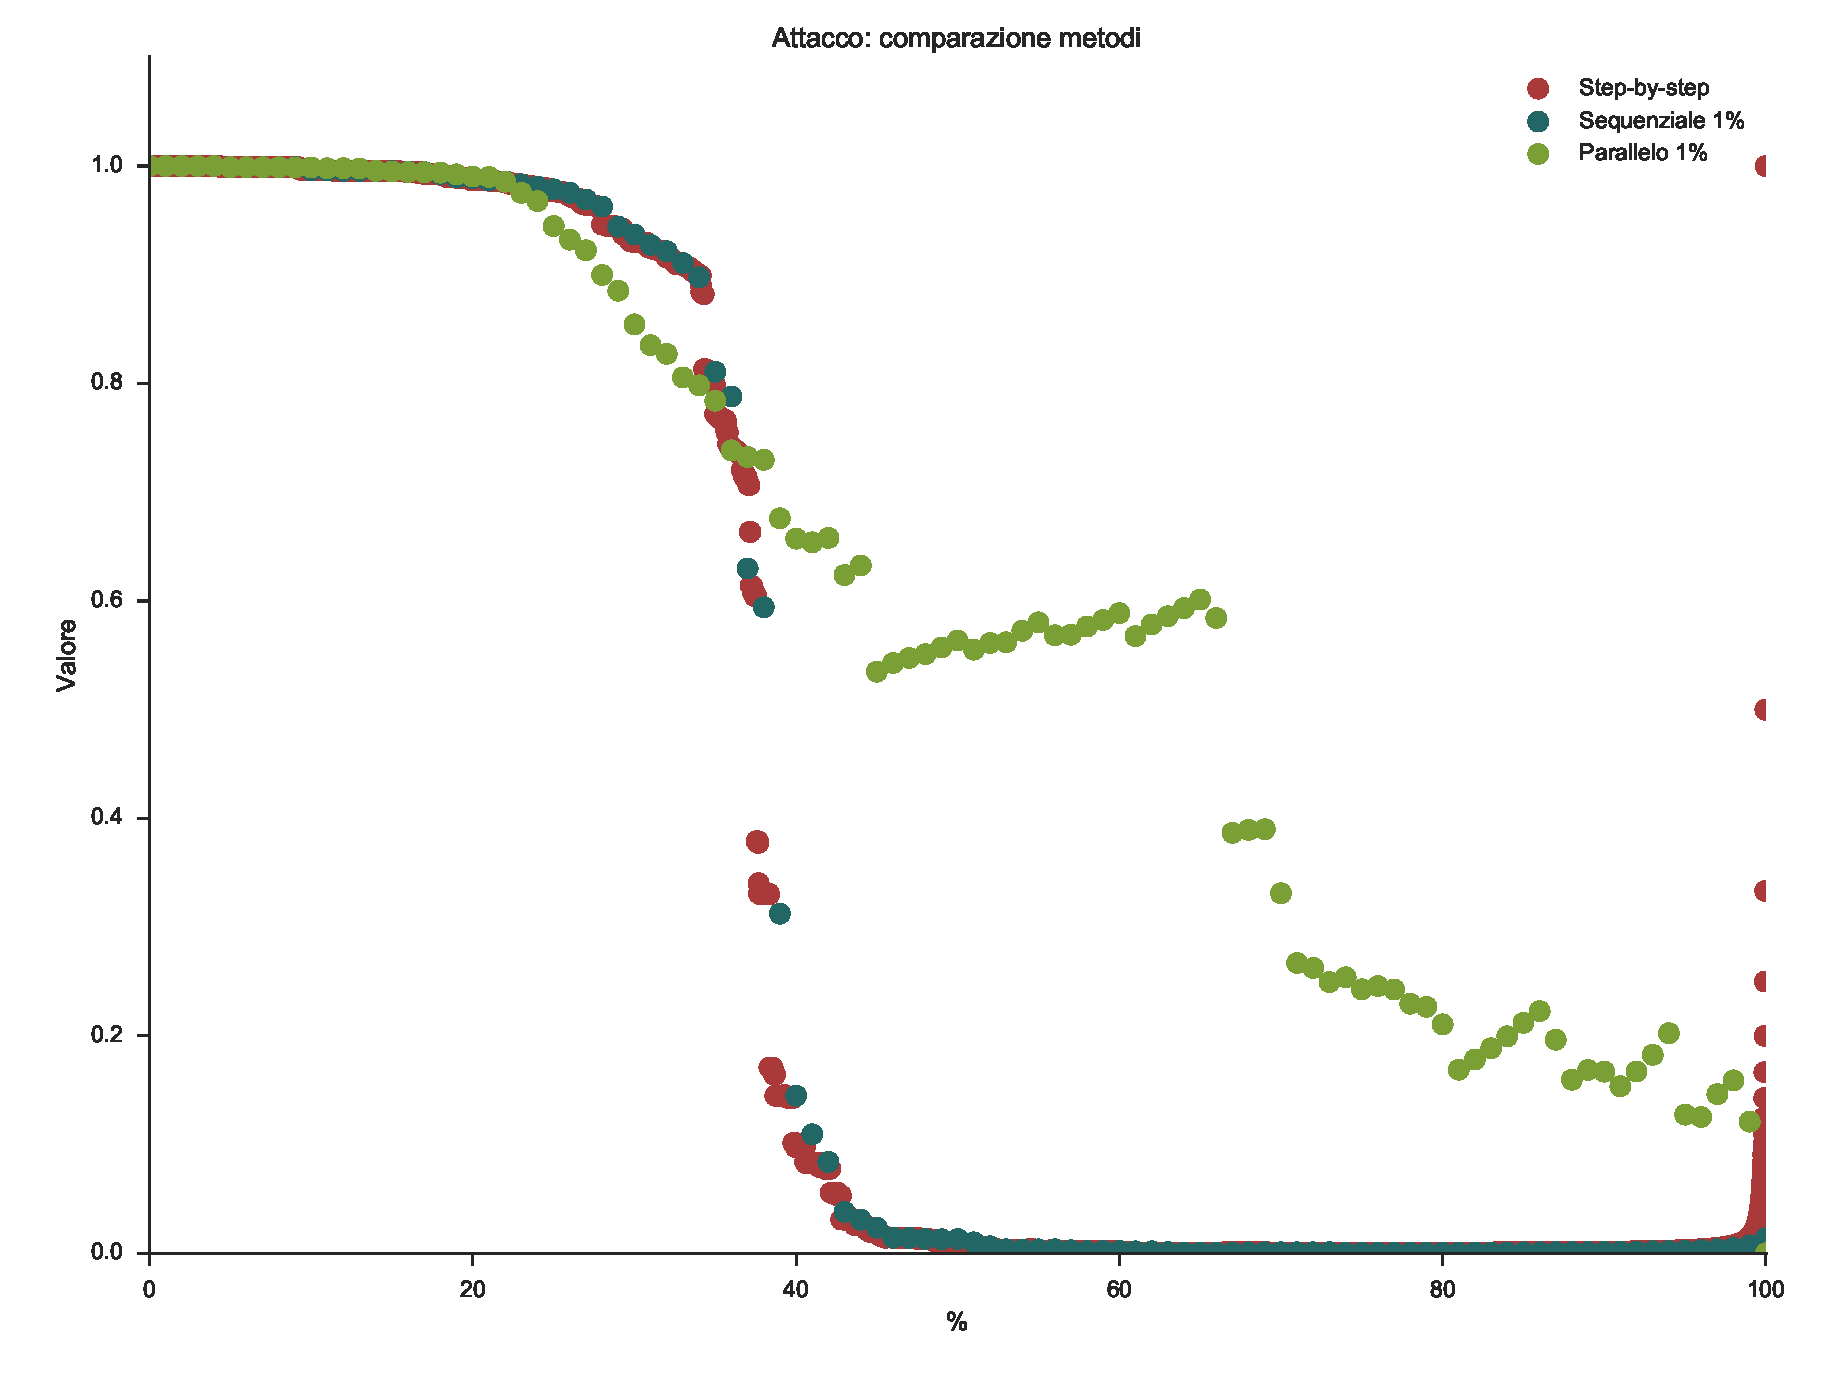
\includegraphics[width=0.65\textwidth]{./Immagini/Attack/AttackGC_Compare}
	\caption[Confronto metodi.]{Confronto sugli effetti dei tre metodi di attacco sulla dimensione del giant cluster.}
	\label{fig:compattack}
\end{figure}

Tale strategia può essere evidenziata solo da una simulazione \textbf{sequenziale}, attuata facendo evolvere la rete passo per passo, secondo una strategia di \emph{steepest descent}. Questo garantisce di trovare la strategia ottimale, soprattutto se vengono inclusi anche gli effetti a cascata dovuti all'overload e alla saturazione di banda. Dal grafico sottostante (attacco intenzionale) si evince comunque che non c'è molta differenza tra procedere sequenzialmente con un campionamento all'1\% o eseguire una simulazione di attacco nodo per nodo, per cui ad ogni modo il costo computazionale complessivo non risulta eccessivo.

Nel caso di random failure (escludendo gli effetti di saturazione a cascata) non c'è invece alcuna differenza tra l'approccio sequenziale e quello \textbf{parallelo}, rendendo il secondo algorimo preferibile nel caso si voglia sfruttare tutta la potenza delle moderne CPU \emph{multicore}.

Riassumendo: 
\begin{itemize}
 \item Nel caso di intentional attack è doveroso usare un approccio sequenziale. 
 \item Nel caso di random failure è consigliabile utilizzare un approccio parallelo.
\end{itemize}

\subsection{Speedup del codice (parte 2: graph-tool)}
Come già detto la prima soluzione al problema dei tempi è stata tentare una parallelizzazione del codice in python: dato che networkx non supporta il calcolo parallelo interno, si è tentato di parallelizzare le funzioni di attacco intenzionale e random failure. Abbiamo però mostrato come alcuni degli algoritmi siano intrinsecamente sequenziali.

Un possibile metodo per ovviare a ciò sarebbe potuto essere generare e salvare in memoria tutte le reti a tutte le iterazioni e successivamente usare delle funzioni parallelizzabili per l'analisi. Tuttavia con networkx la richiesta di tempo di calcolo rimane comunque alta e si aggiungerebbe anche il problema della memoria RAM, dello spazio su disco e dei tempi di lettura e scrittura.

L'unica via praticabile è stata ripiegare su \emph{graph-tool}: un'altra libreria meno \emph{user-friendly} ma estremamente più efficiente e sopratutto impostata di default sul calcolo parallelo. Le funzioni di analisi topologica e statistica sono molto più veloci rispetto a networkx, poiché implementate in C con il \emph{template programming} ed ottimizzate in fase di compilazione. Inoltre la possibilità di usarle nativamente in parallelo su 4 core e 8 thread ci ha permesso di calcolare le singole funzioni con una velocità più di 60 volte superiore a prima.

Considerato ciò, il codice per lo studio percolativo delle reti è stato convertito (con non poco sforzo) per poter fare uso della nuova libreria. Alla fine, per l'analisi percolativa completa di tutte le reti, ovvero con lo studio, in funzione dei nodi rimossi, delle quantità 

\begin{itemize}
 \item   diametro $D$
 \item   average path lenght $\langle l \rangle$
 \item   clustering coefficient $C$
 \item   average degree $\langle k \rangle$
 \item   dimensioni del giant cluster
 \item   criterio di soglia percolativa (andamento di $\langle k^2 \rangle / \langle k \rangle$)
\end{itemize}

da una previsione iniziale di più di 24 ore di tempo di calcolo si è passati a circa $3/4$ d'ora, con uno speedup di circa un fattore 30.

\begin{figure}[h!]
	\centering
	
\includegraphics[width=0.55\textwidth]{./Immagini/Attack/meme_Obama.jpg}
\end{figure}

\subsection{Random failure}
Le reti da cui è partito lo studio percolativo sono le 5 definite e costruite nel precedente paragrafo. Le grandezze iniziali erano:


\begin{table}[ht!]
\centering
% \caption{Dati iniziali delle reti studiate.}
	\begin{tabular}{cccccccccc}
	\toprule
	Rete		&N		&$GC\%$	&$D$	&$\langle l\rangle$	&$C$		&$\langle k\rangle$	&$C/\langle k\rangle$	&$\langle k^2\rangle/\langle k\rangle$	&$f\%$\\
	\midrule  
	Tim		&1756	&1		&2	&1.96			&0.89	&64.3			&0.014				&359							&99.7\\
	Vodafone	&1771	&1		&2	&1.97			&0.87	&52.9			&0.016				&243							&99.6\\
	Wind		&2365	&1		&2	&1.96			&0.89	&97.3			&0.009				&478							&99.8\\
	Tre		&1395	&1		&2	&1.97			&0.88	&41.4			&0.021				&239							&99.6\\
	Roma		&7287	&1		&2	&1.97			&0.89	&239.1			&0.004				&1353							&99.9\\
	\bottomrule
	\end{tabular}
\caption{Grandezze topologiche e statistiche delle reti a $t=0$}
\label{tab:datiInitial}
\end{table}

La prima cosa da notare è che le reti delle singole compagnie hanno un rapporto coefficiente di clustering-grado medio in linea con molte altre reti reali \parencite{Barbalbert2002}, e che la rete costruita con tutte le antenne non vede aumentare particolarmente il suo clustering. Inoltre ci si aspetta che le reti siano tutte particolarmente resistenti sotto random failure, comportamento che sembra più simile a quello di una rete scale free. Tuttavia una rete random con un grado medio alto ha comunque un $f$ molto alto. Per esempio, una rete random avente $N = N_{Tim}$ e $\langle k \rangle = \langle k \rangle_{Tim}$, avrebbe una $f$ critica di poco inferiore: $\sim 98\%$. Infatti, essendo per una rete random $\langle k \rangle = Np$, perché sia uguale a $\langle k \rangle_{Tim}$ con $\sim 1800$ nodi, deve essere $p \sim 3.7\%$, 
$$\Rightarrow \sigma^2 = Np(1-p) = \langle k^2 \rangle - \langle k \rangle^2 \sim 62$$
$$\Rightarrow \frac{\langle k^2 \rangle }{\langle k \rangle} = \frac{Np(1-p)-(Np)^2}{Np} \sim 1+Np = 1+ \langle k \rangle \sim 65$$
$$\Rightarrow f \sim 1 - \frac{1}{65} \sim 98\%$$

Con una rete random costruita con i parametri della rete totale si ottiene $f = 99.5$. Valori quindi che si distinguono poco dalla soglia per una rete power-law finita, anche nel caso in cui l'esponente sia di poco maggiore di 3: $f \sim 1 - \frac{1}{\frac{\gamma - 2}{\gamma-3}k_{max}} > 90\%$ già per un grado massimo di $\sim10$.


\subsubsection{Attacco intenzionale}
Nello scenario di attacco intenzionale ci si aspetta una veloce frammentazione della rete. I cluster diverranno rapidamente più piccoli fino a frammentarsi del tutto entro pochi punti percentuali di nodi rimossi. Nel caso di una rete fortemente connessa come quella in esame ci si aspetta una resistenza maggiore, ma comunque una soglia percolativa bassa (approssimativamente entro il $50\%$). Se la rete è di tipo scale-free dovrebbe essere più fragile ad attacchi di questo tipo: mentre in una rete random i nodi più connessi sono solo una coda della distribuzione del grado; una rete a power-law ha in proporzione molti più nodi molto connessi.

Dal punto di vista del diametro della rete, levando i nodi più connessi ci si aspetta che esso aumenti fino a quando la rete diventa tanto frammentata da essere costituita da cluster con pochissimi nodi. Oltrepassata la soglia di frammentazione quindi il diametro dei cluster più grandi decrescerà rapidamente a zero.
\clearpage
\subsection{Risultati}
\begin{figure}[hb!]
	\centering
	\subfloat[$GC$]
	{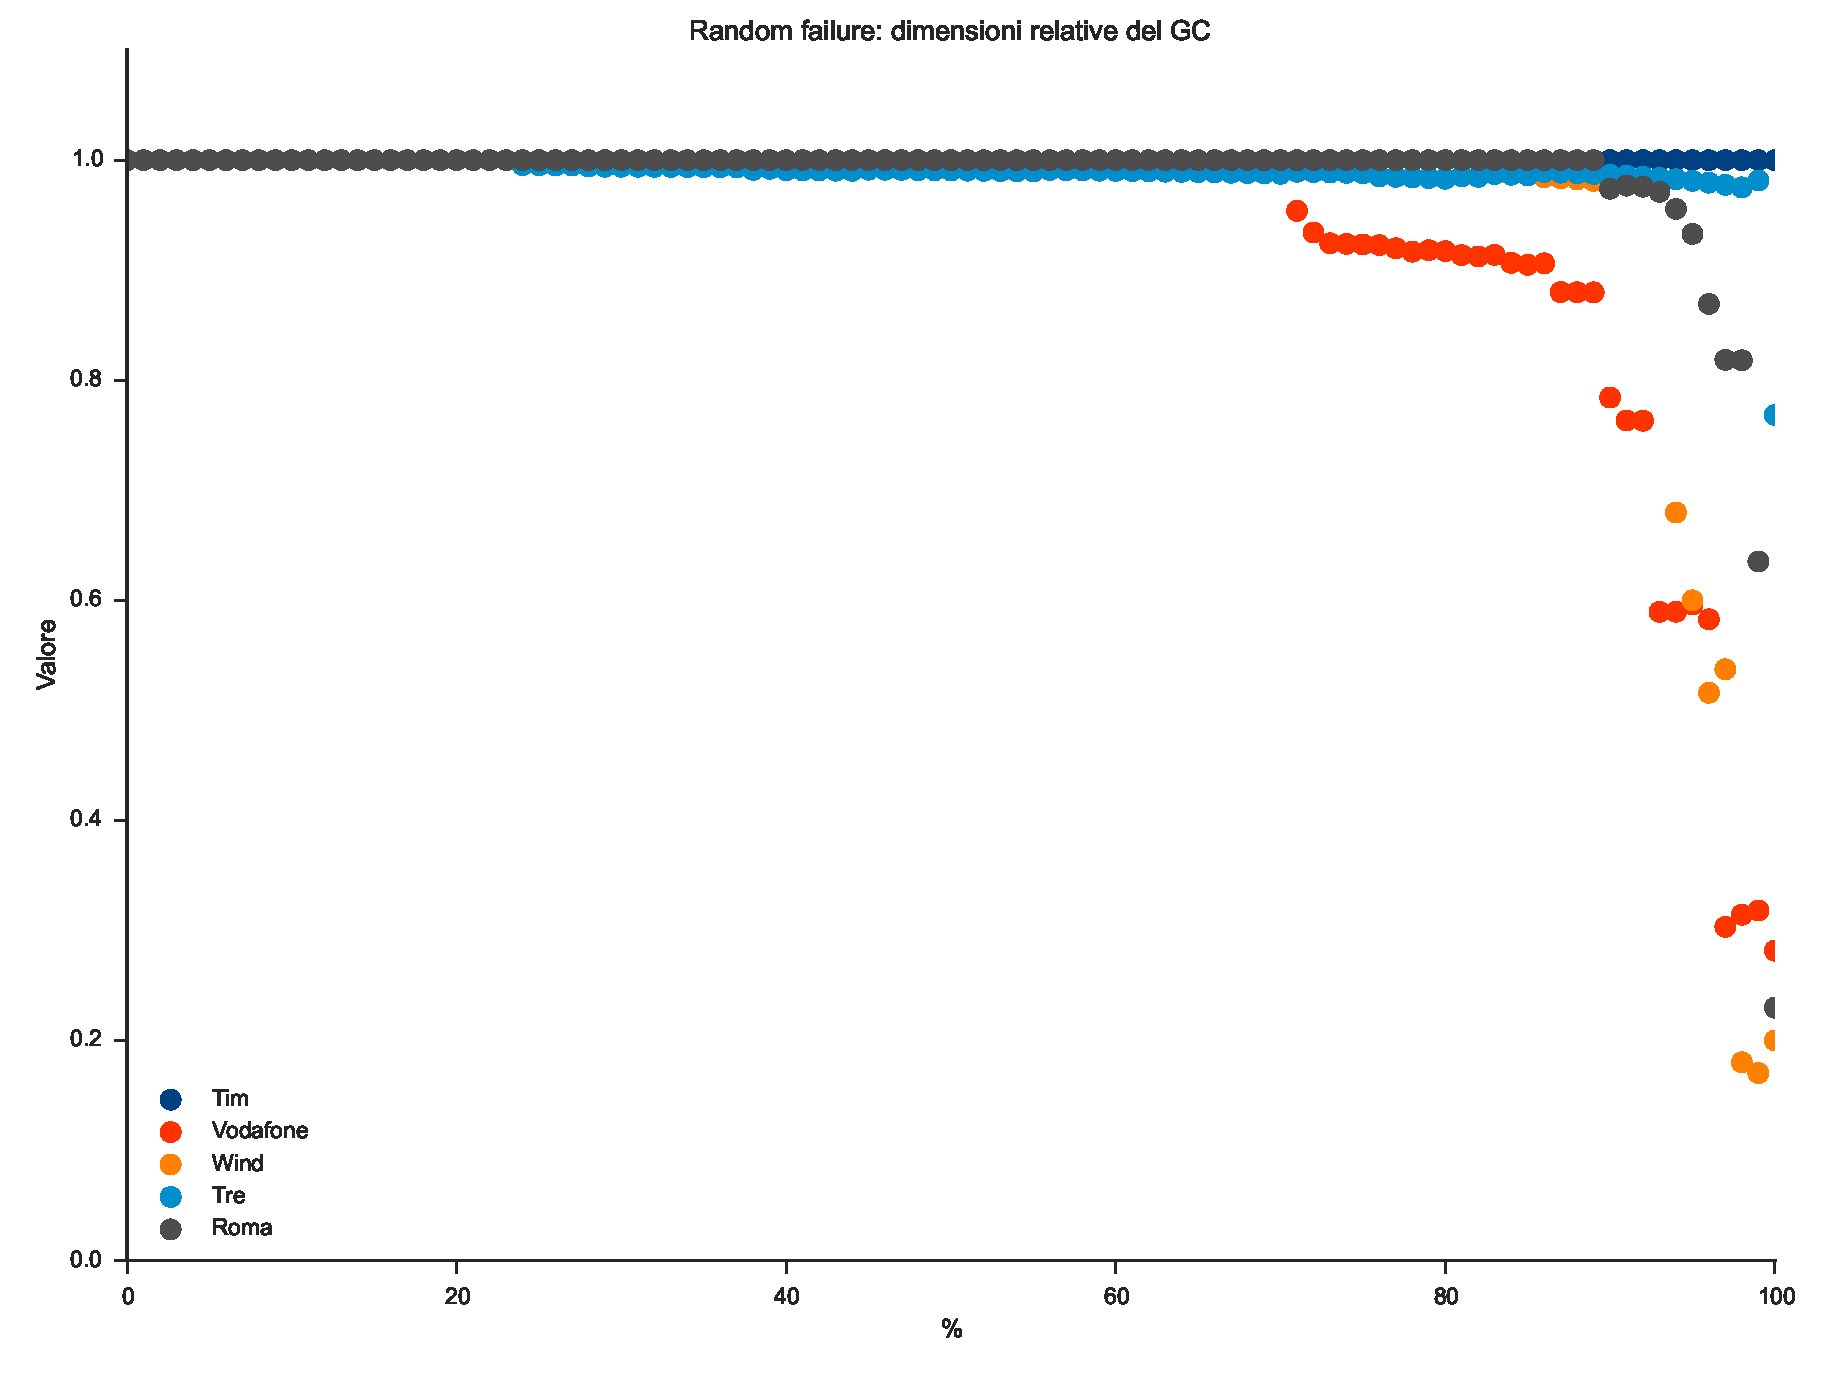
\includegraphics[width=0.47\textwidth]{./Immagini/Attack/gToolFailureGC_Final}}
	$\;$
	\subfloat[$C$]
	{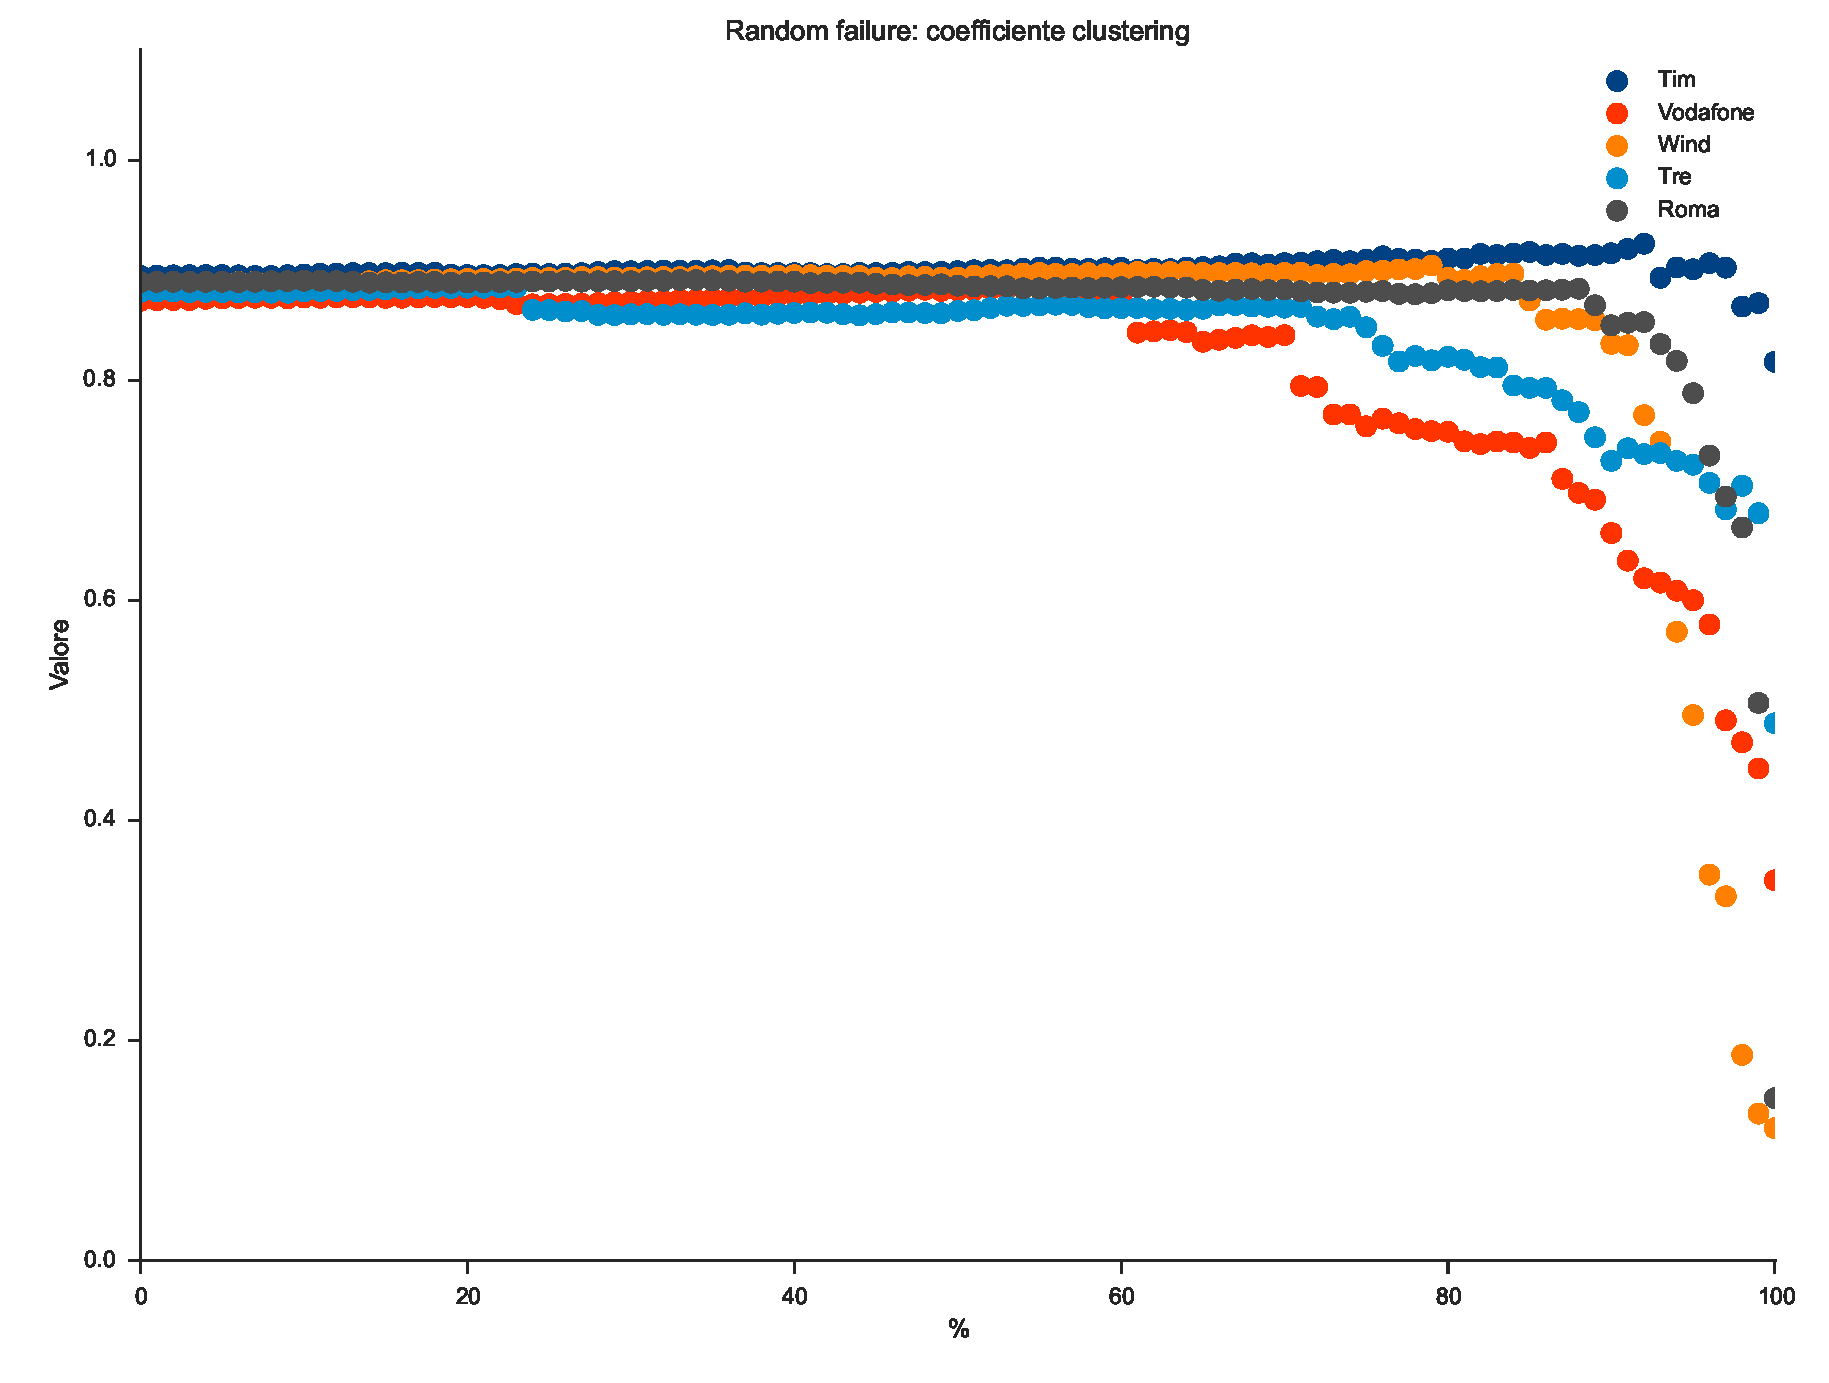
\includegraphics[width=0.47\textwidth]{./Immagini/Attack/gToolFailureC_Final}}
	\\
	\subfloat[$\langle l \rangle$]
	{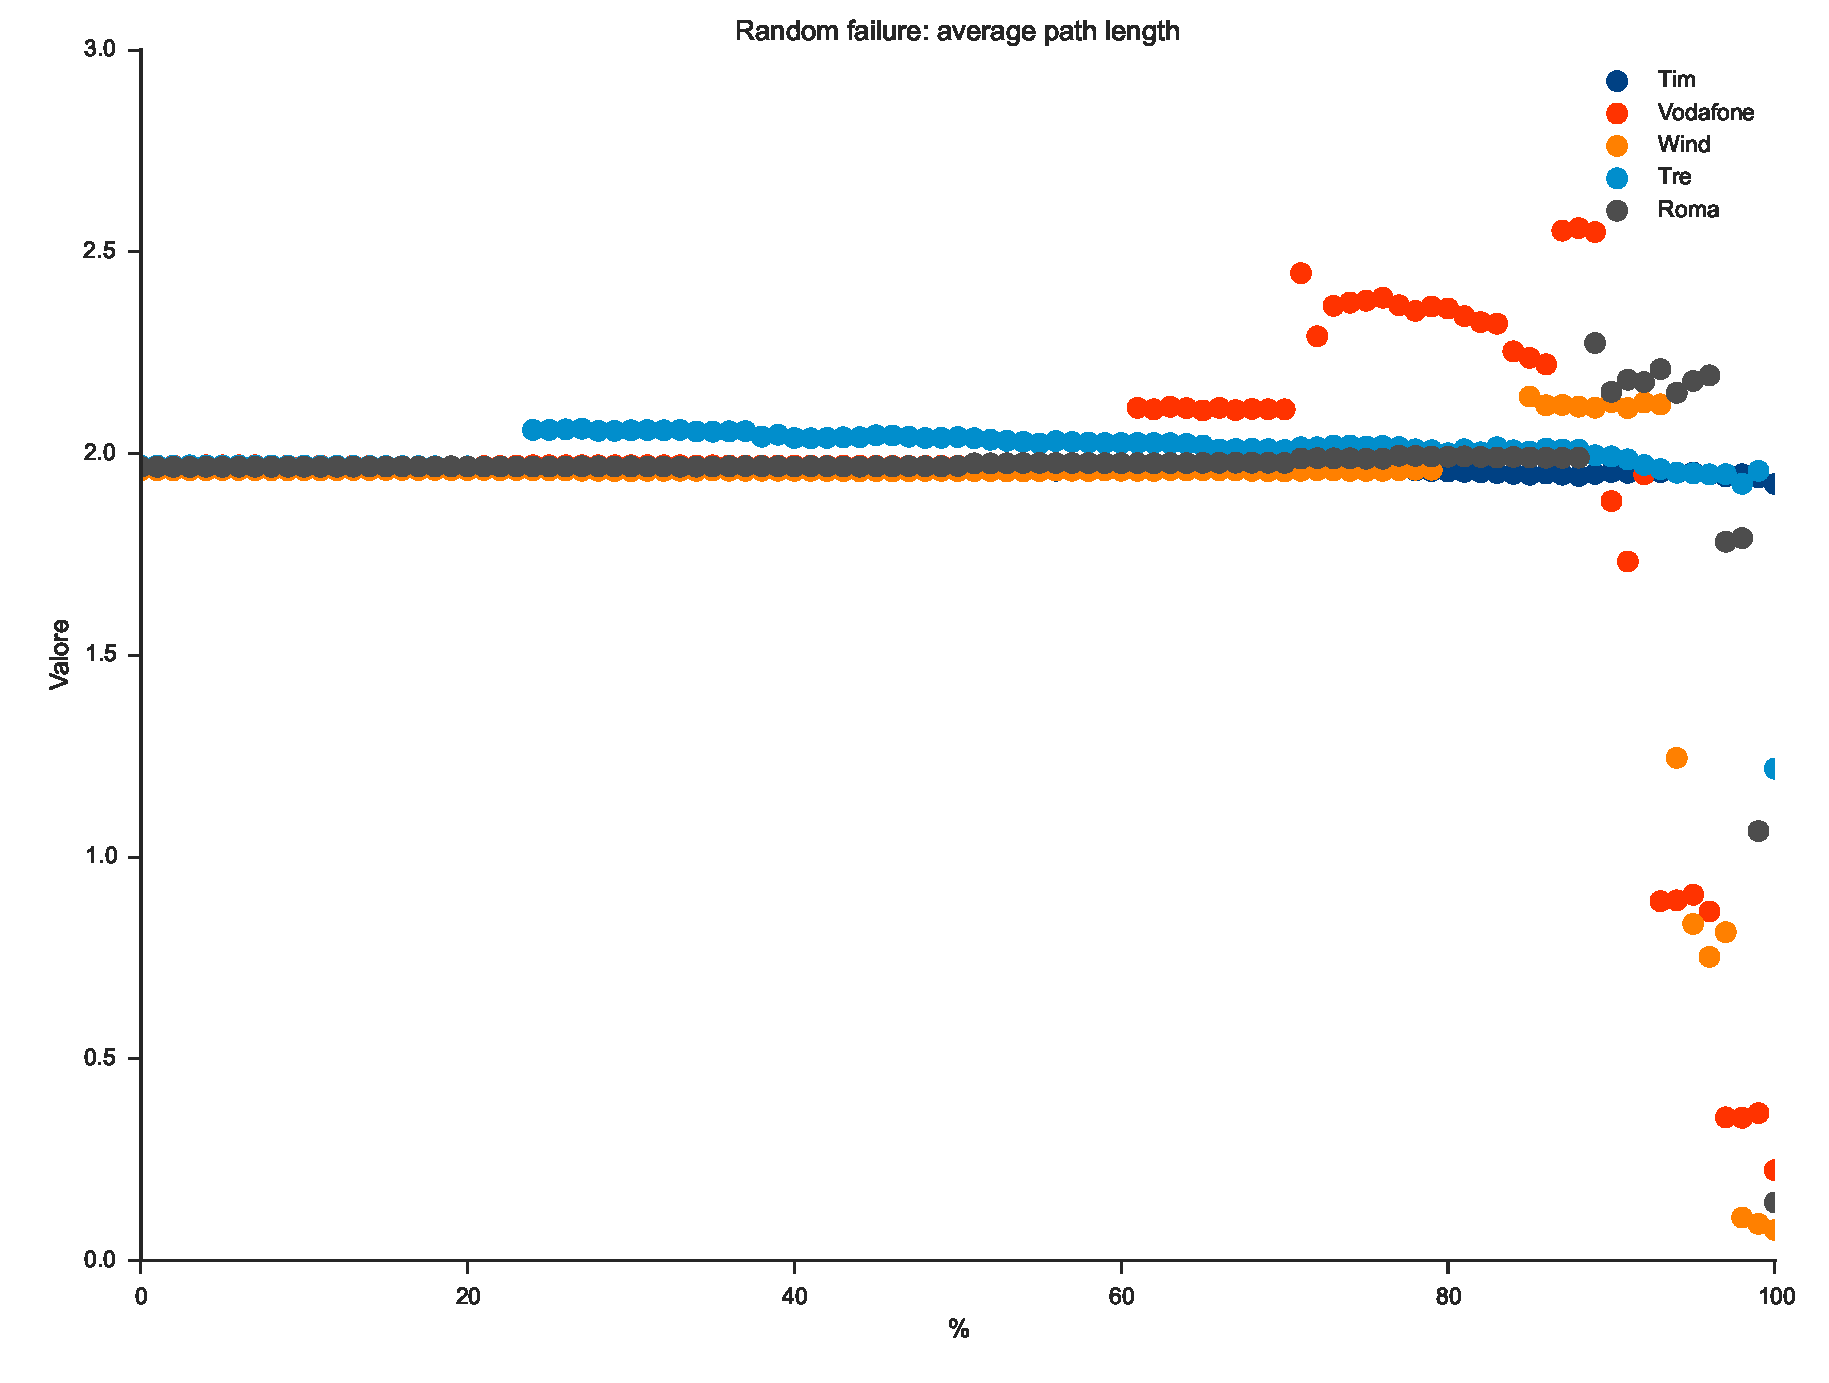
\includegraphics[width=0.47\textwidth]{./Immagini/Attack/gToolFailurel_Final}}
	$\;$
	\subfloat[$D$]
	{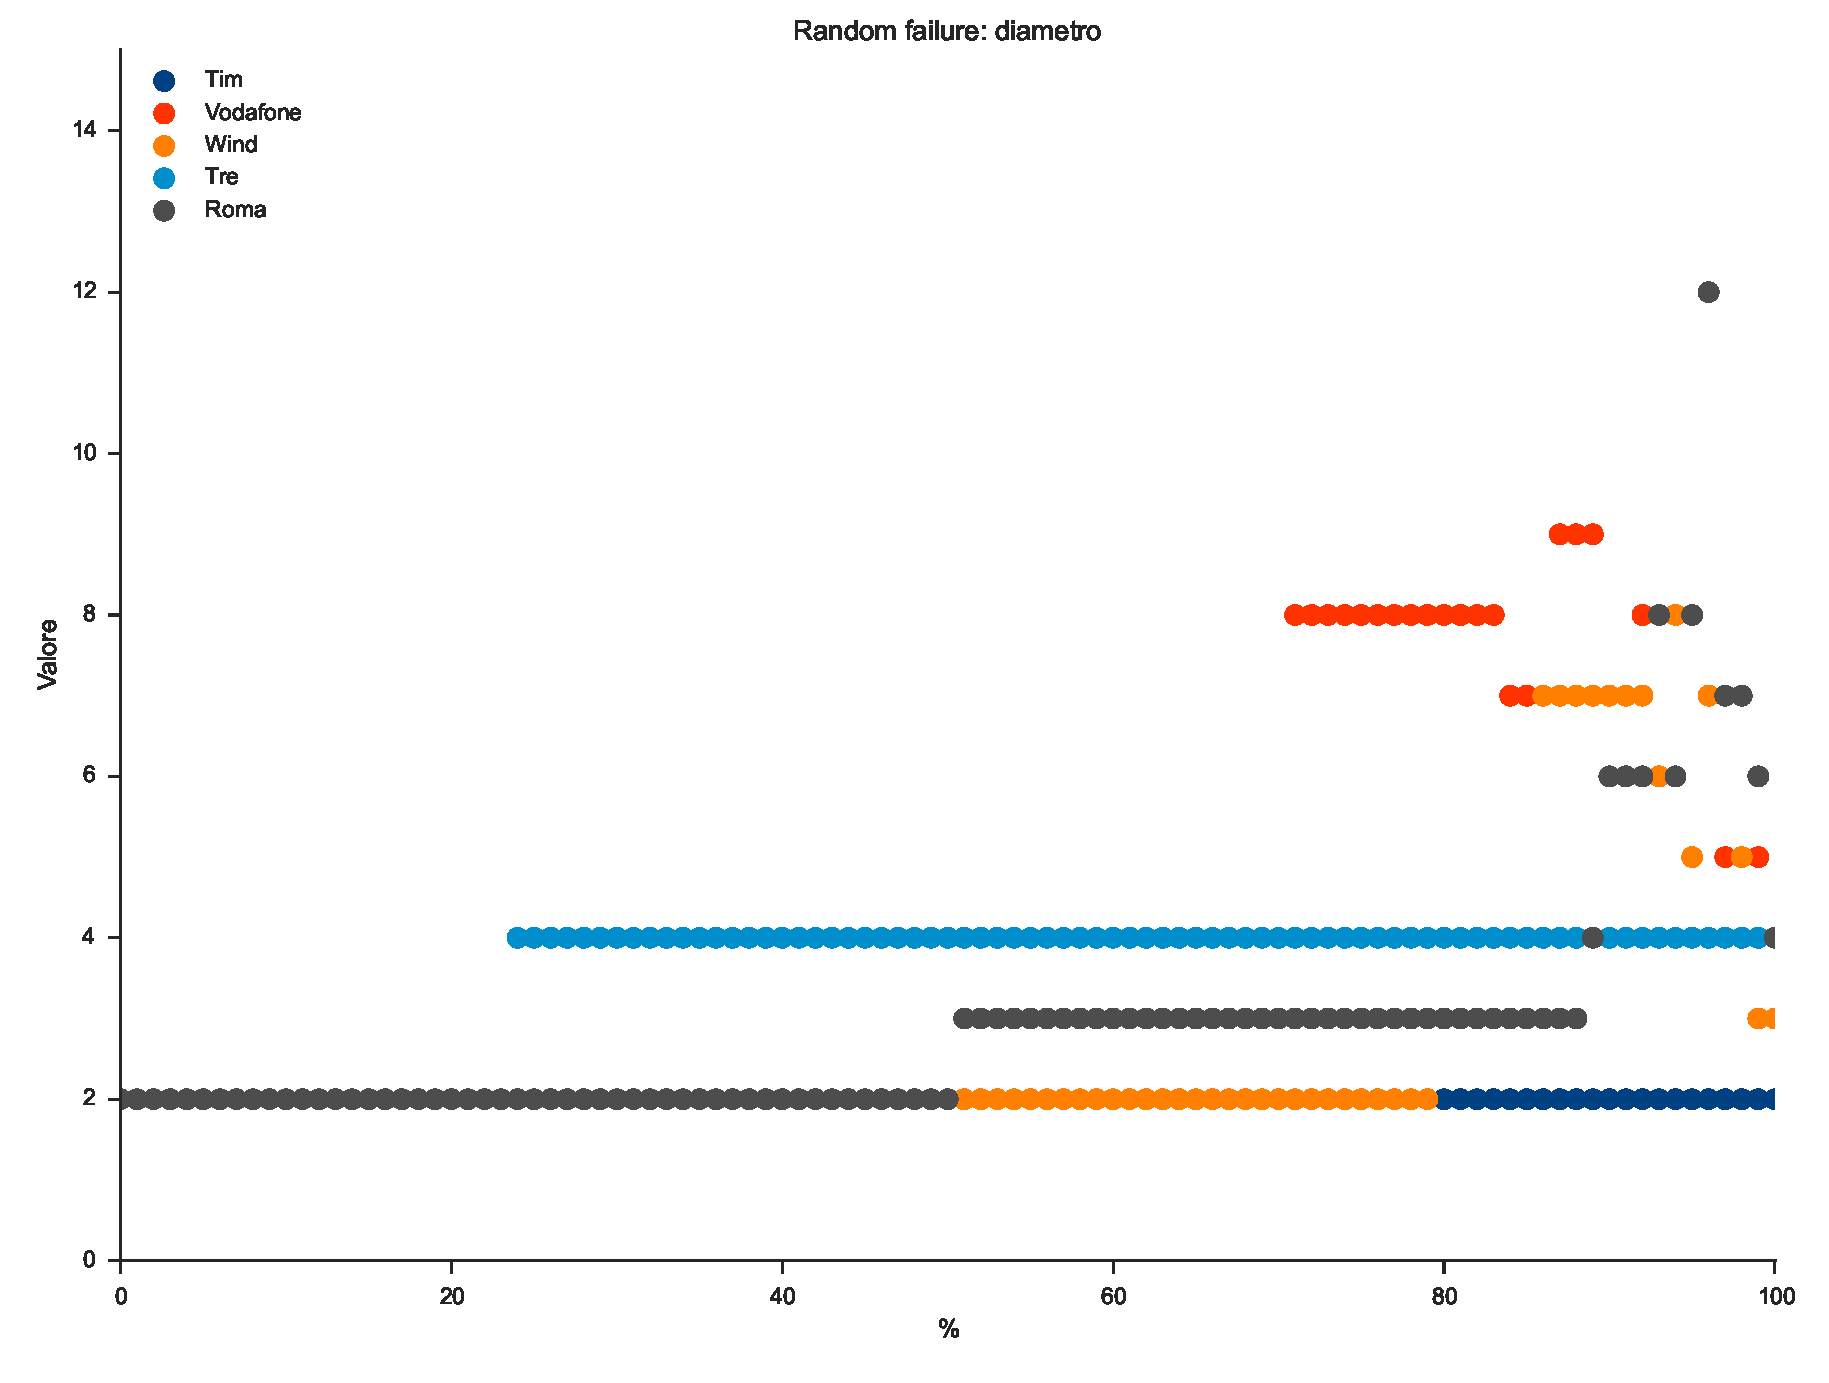
\includegraphics[width=0.47\textwidth]{./Immagini/Attack/gToolFailureD_Final}}
	\\
	\subfloat[$\langle k \rangle$]
	{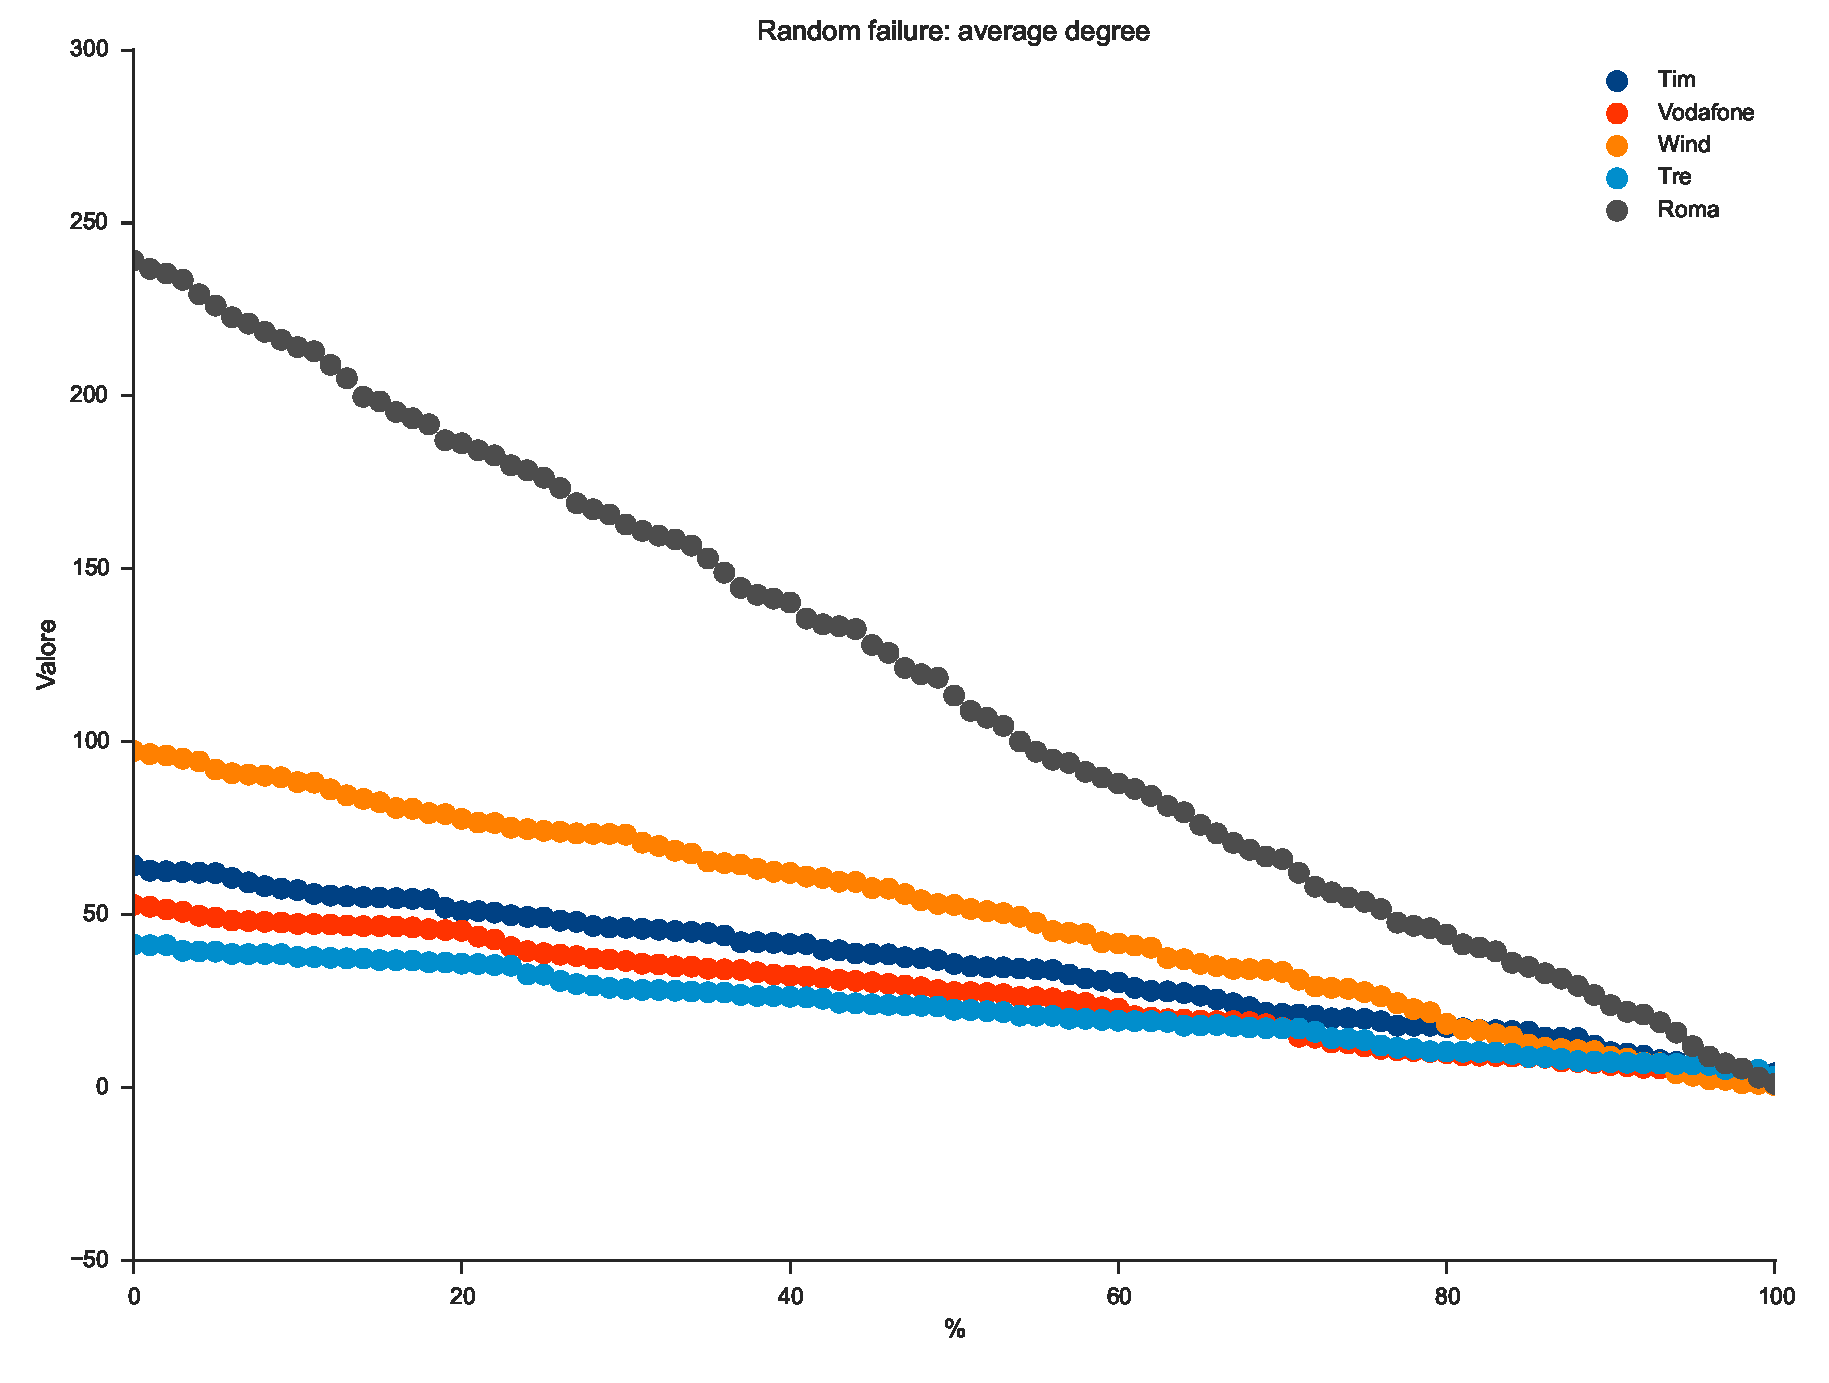
\includegraphics[width=0.47\textwidth]{./Immagini/Attack/gToolFailurek_Final}}
	$\;$
	\subfloat[$\langle k^2 \rangle/\langle k \rangle$]
	{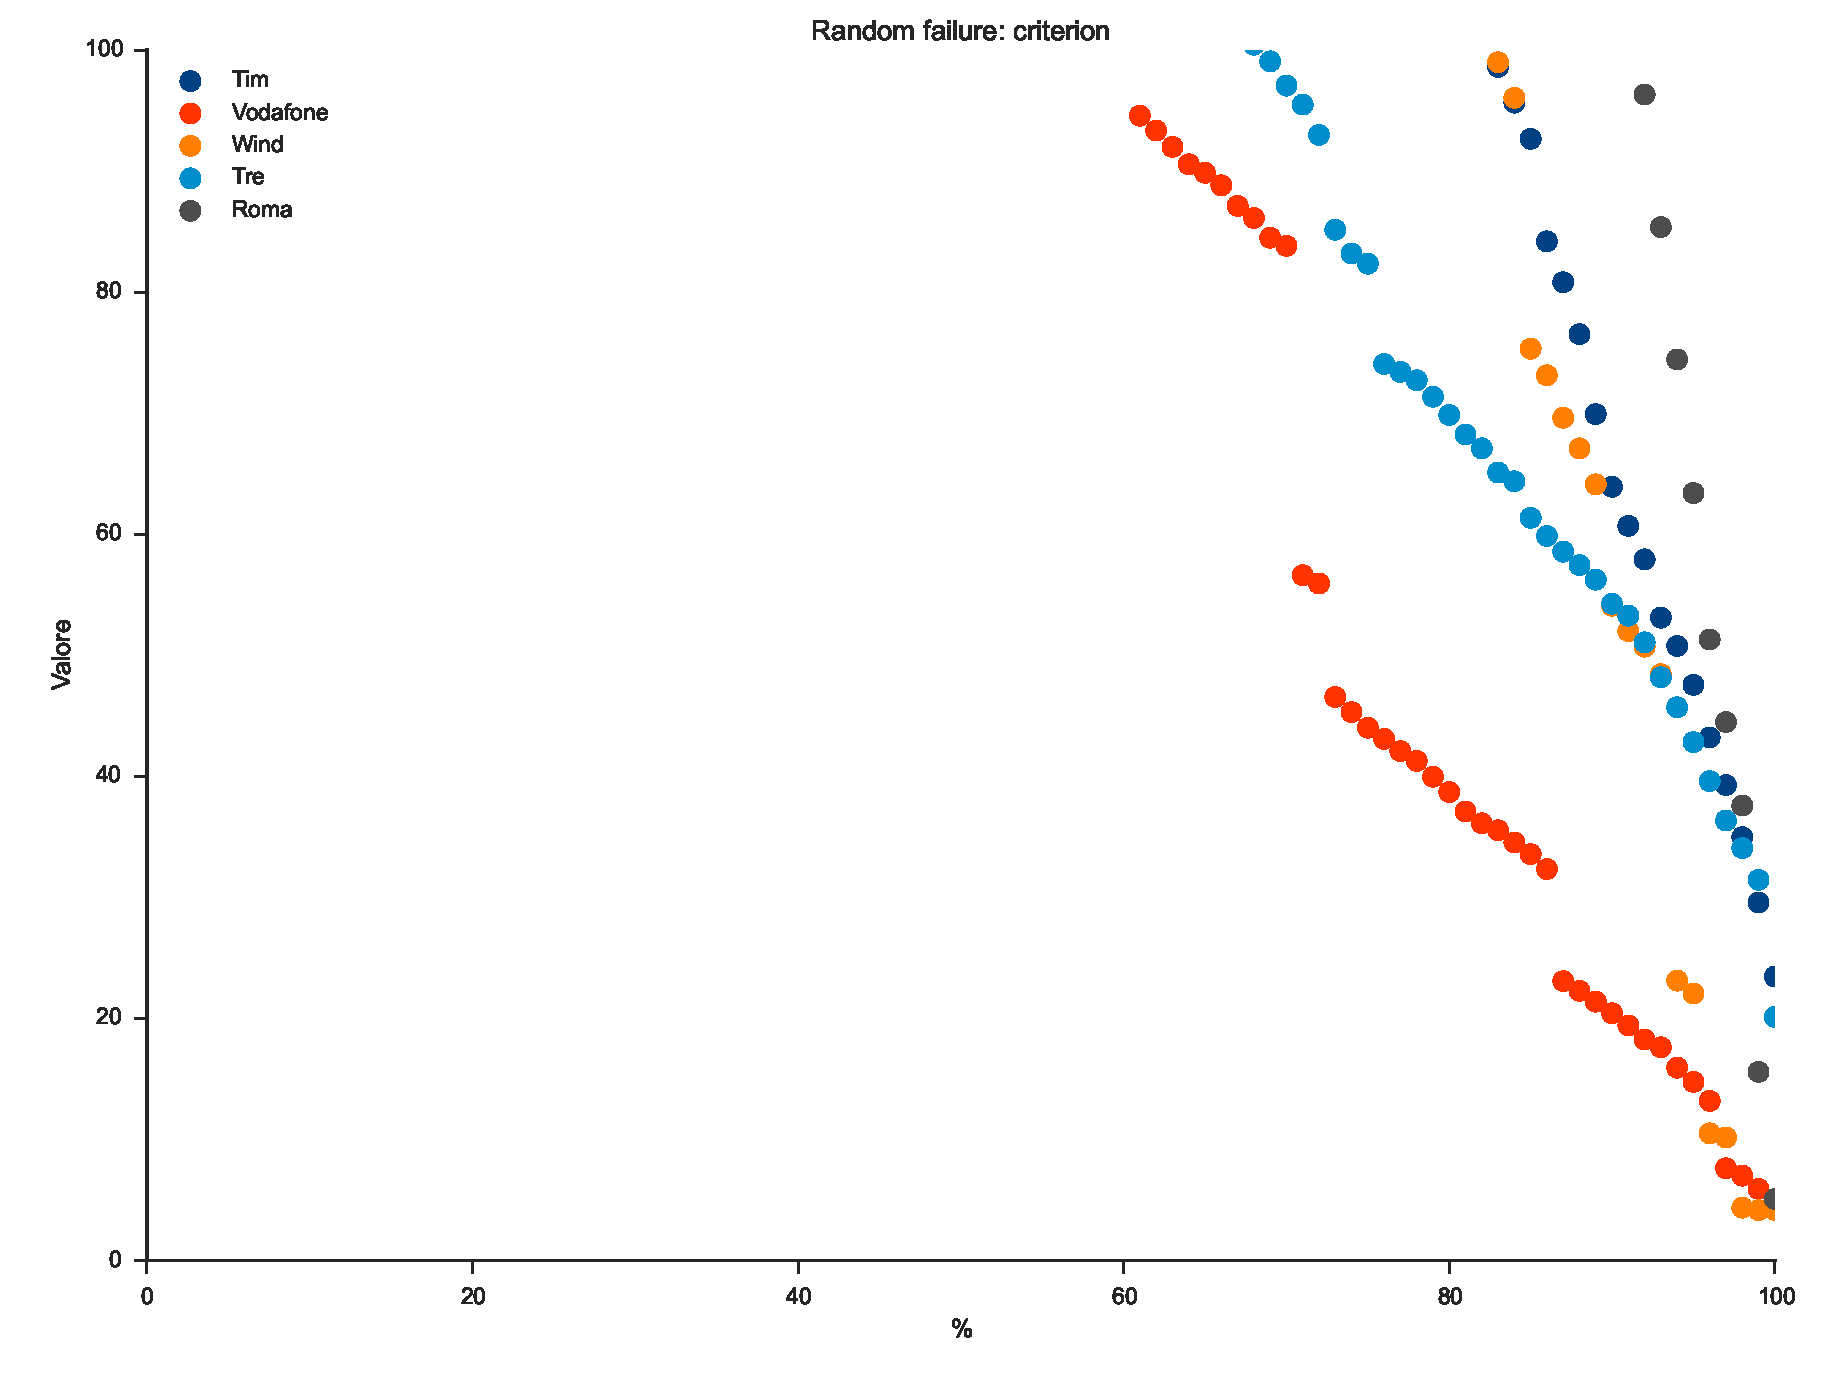
\includegraphics[width=0.47\textwidth]{./Immagini/Attack/gToolFailurec_Final}}
	\caption[Risultati random.]{Risultati per rimozione random}
	\label{fig:fail}
\end{figure}

\begin{figure}[p!]
	\centering
	\subfloat[$GC$]
	{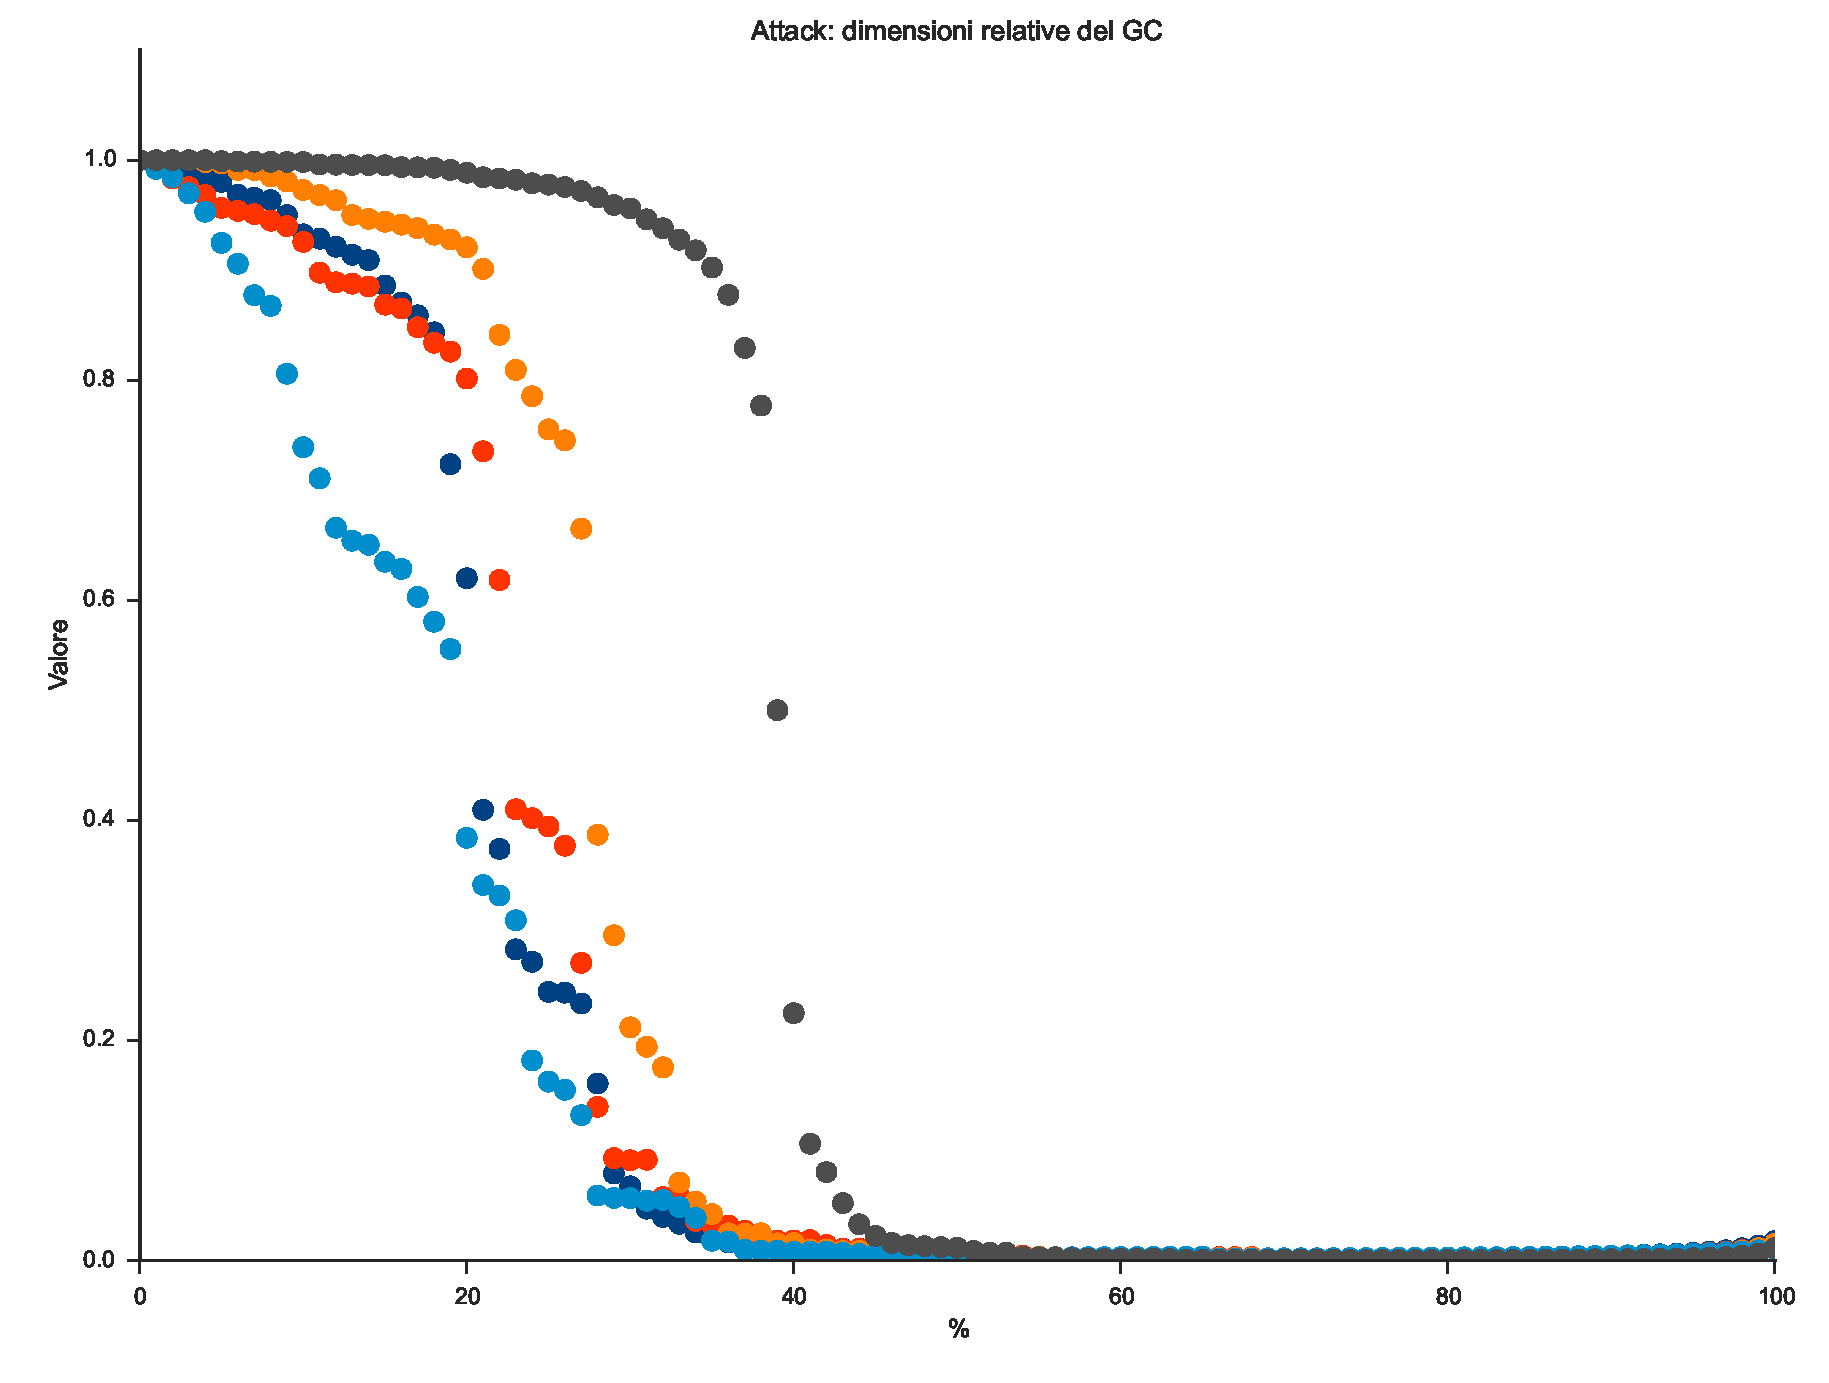
\includegraphics[width=0.47\textwidth]{./Immagini/Attack/gToolAttackGC_Final}}
	$\;$
	\subfloat[$C$]
	{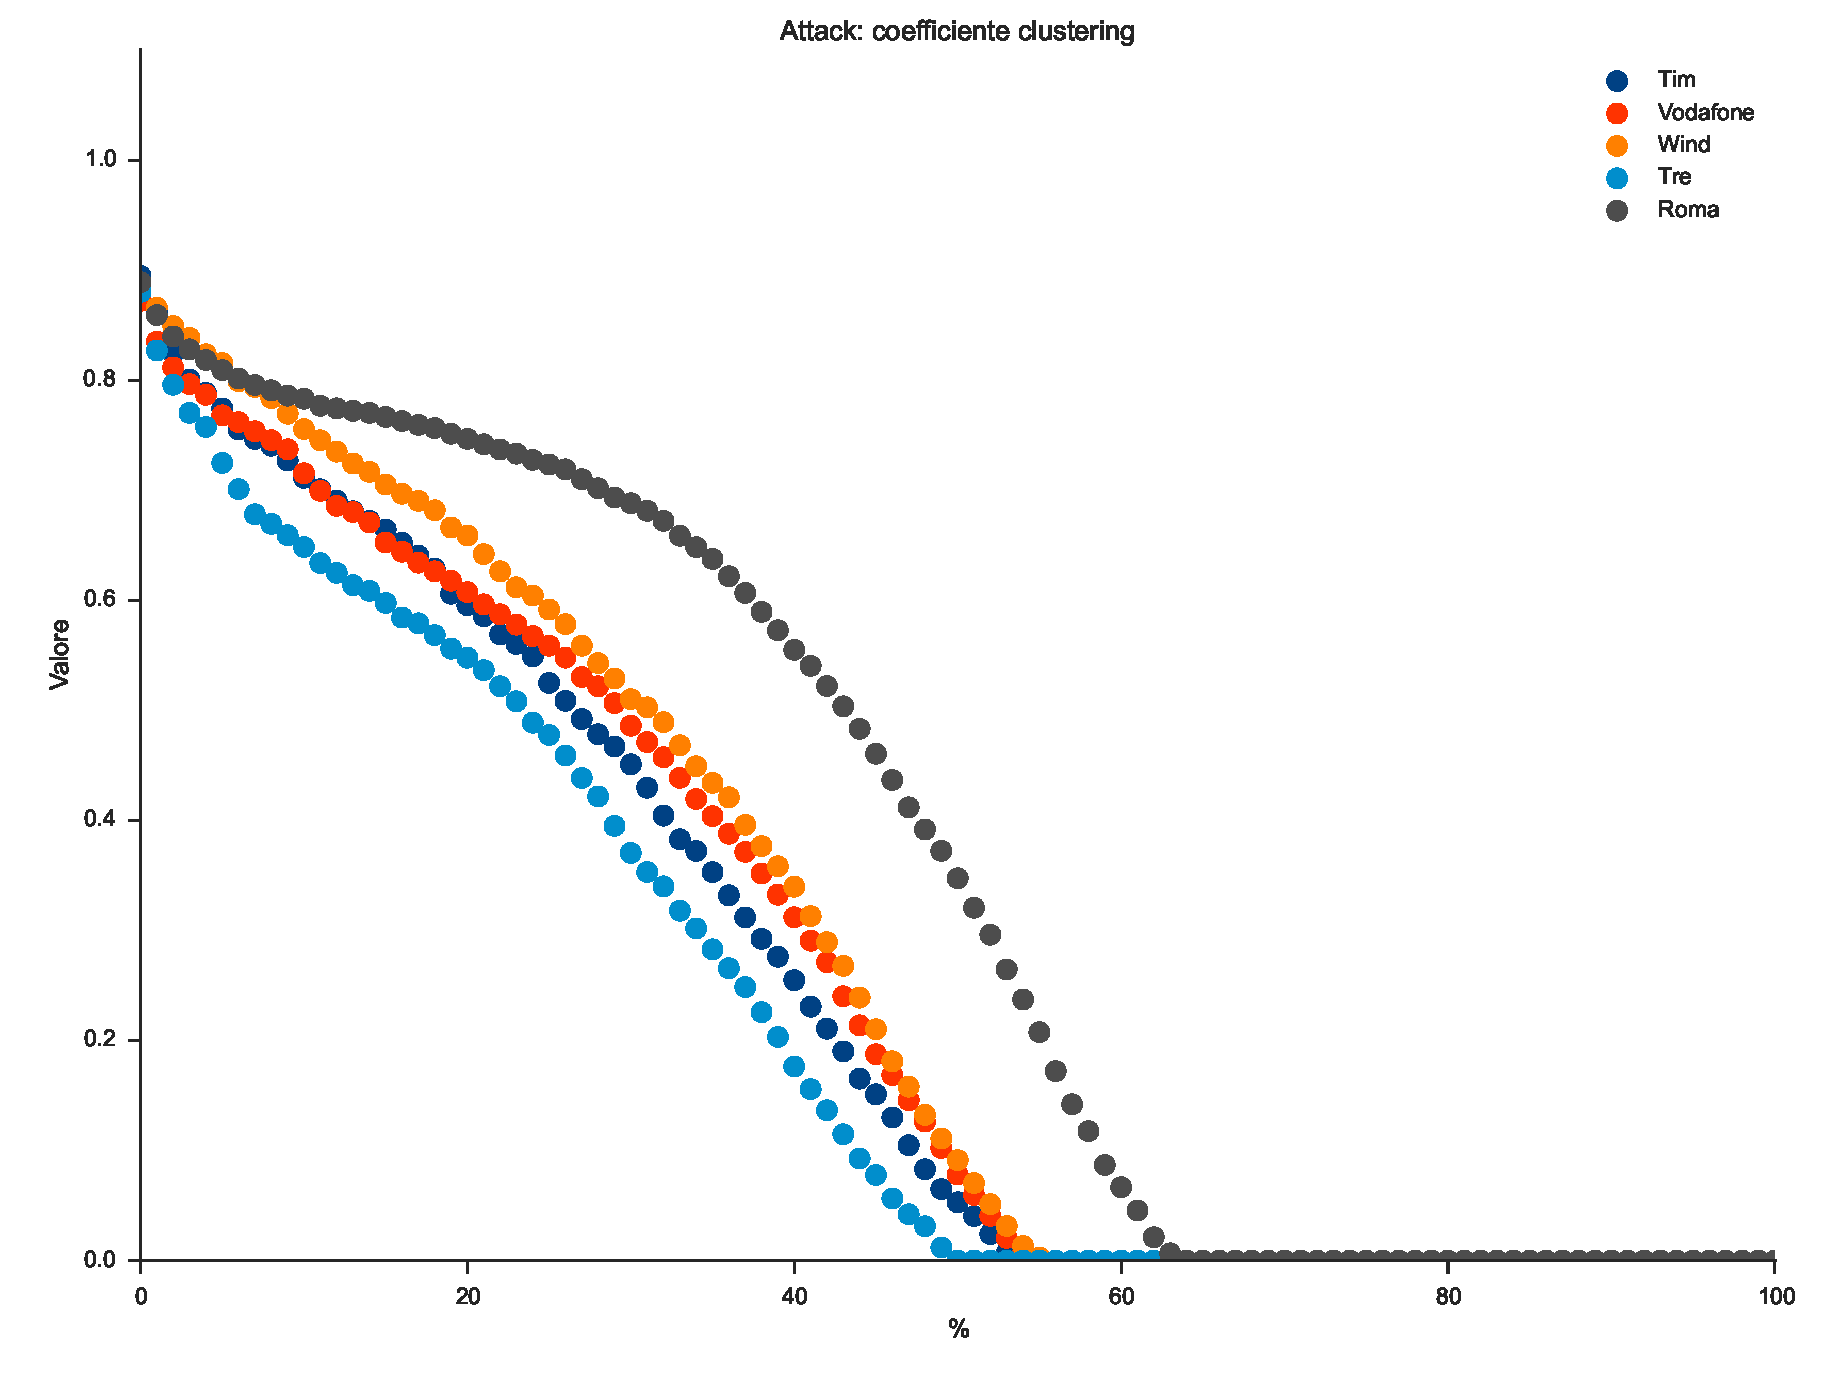
\includegraphics[width=0.47\textwidth]{./Immagini/Attack/gToolAttackC_Final}}
	\\
	\subfloat[$\langle l \rangle$]
	{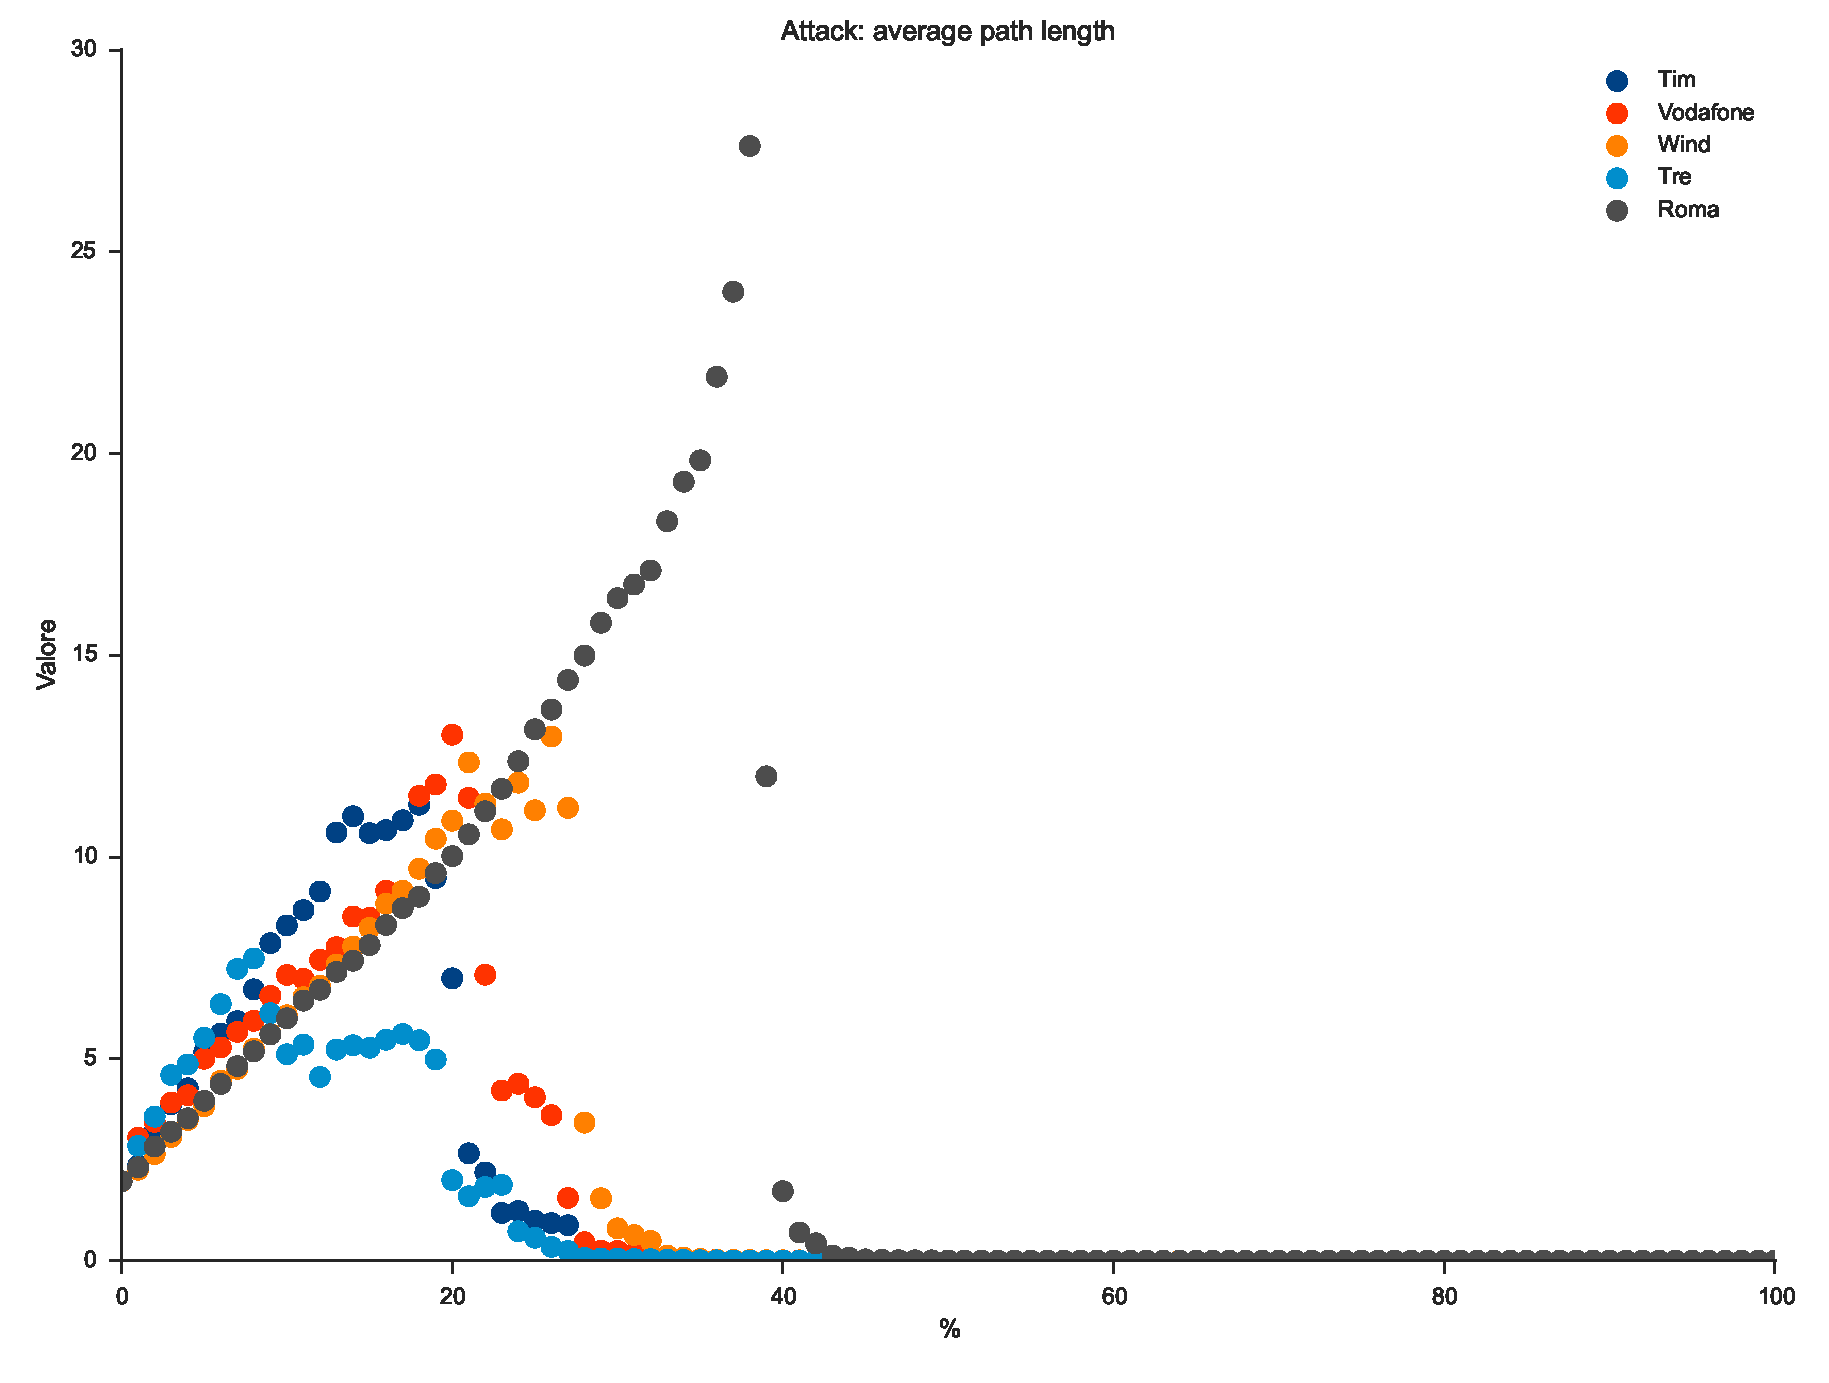
\includegraphics[width=0.47\textwidth]{./Immagini/Attack/gToolAttackl_Final}}
	$\;$
	\subfloat[$D$]
	{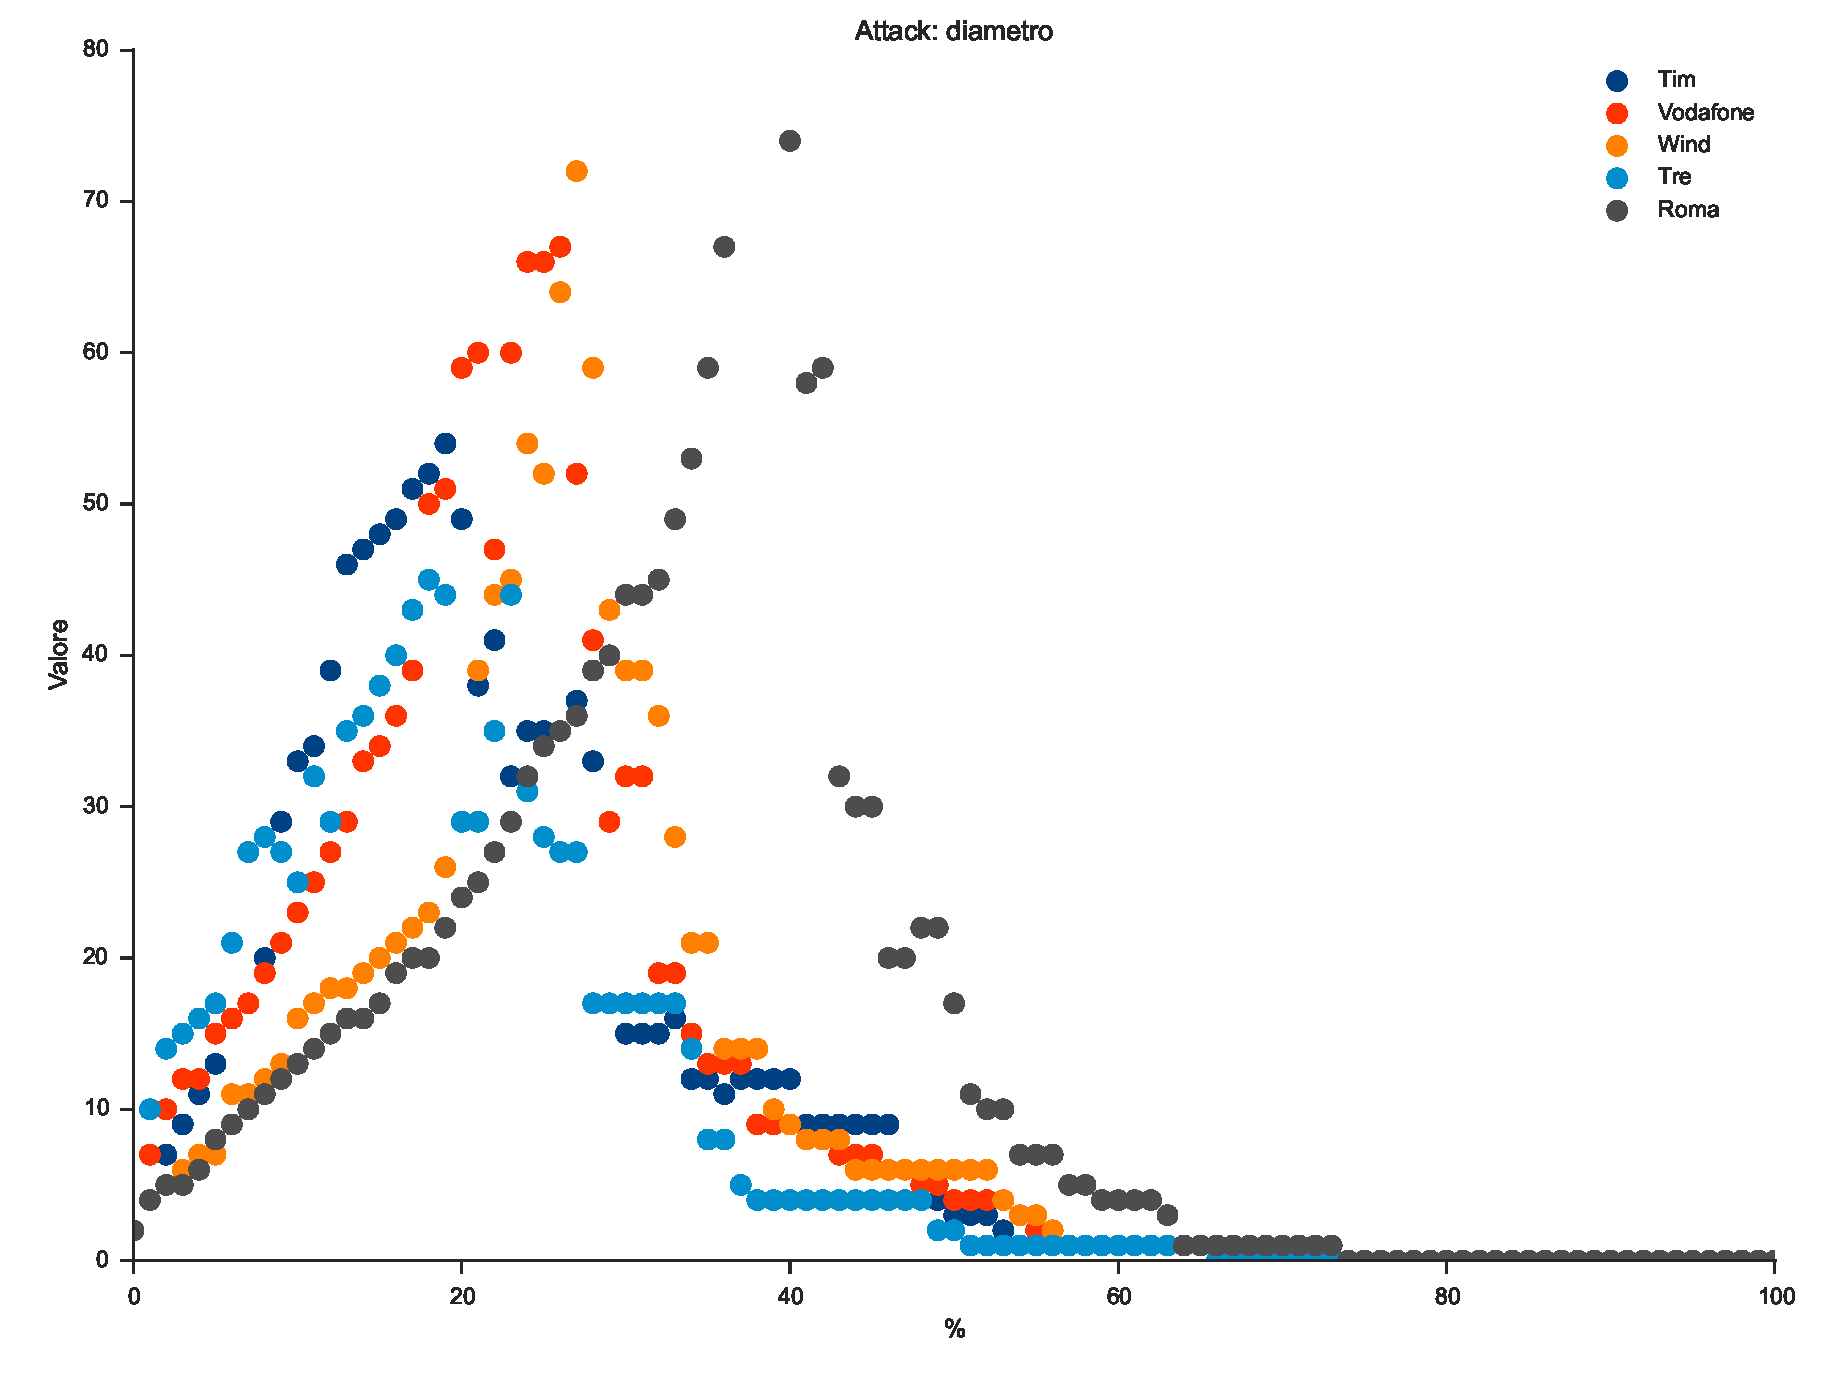
\includegraphics[width=0.47\textwidth]{./Immagini/Attack/gToolAttackD_Final}}
	\\
	\subfloat[$\langle k \rangle$]
	{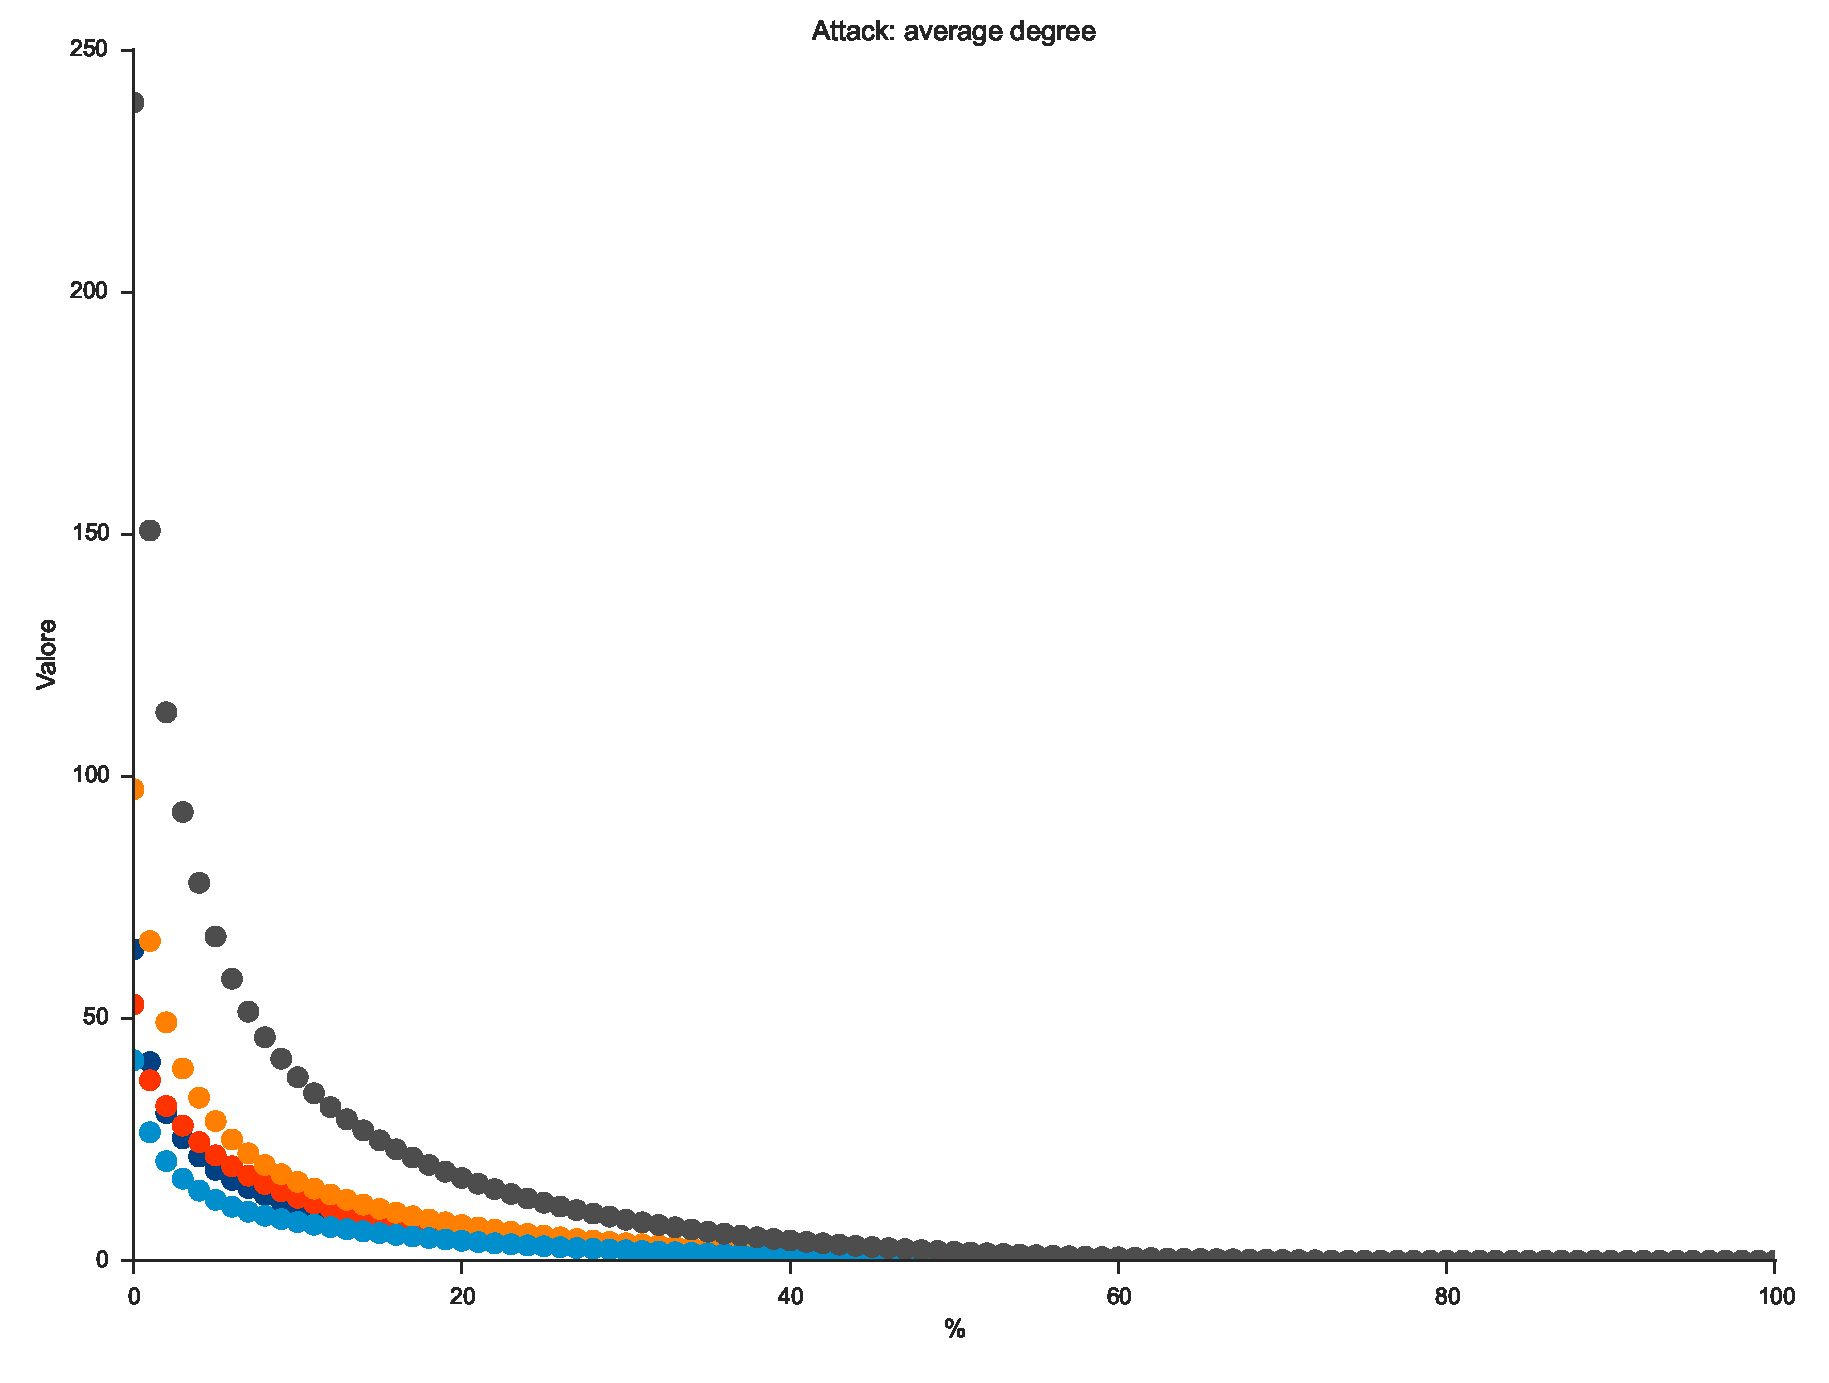
\includegraphics[width=0.47\textwidth]{./Immagini/Attack/gToolAttackk_Final}}
	$\;$
	\subfloat[$\langle k^2 \rangle/\langle k \rangle$]
	{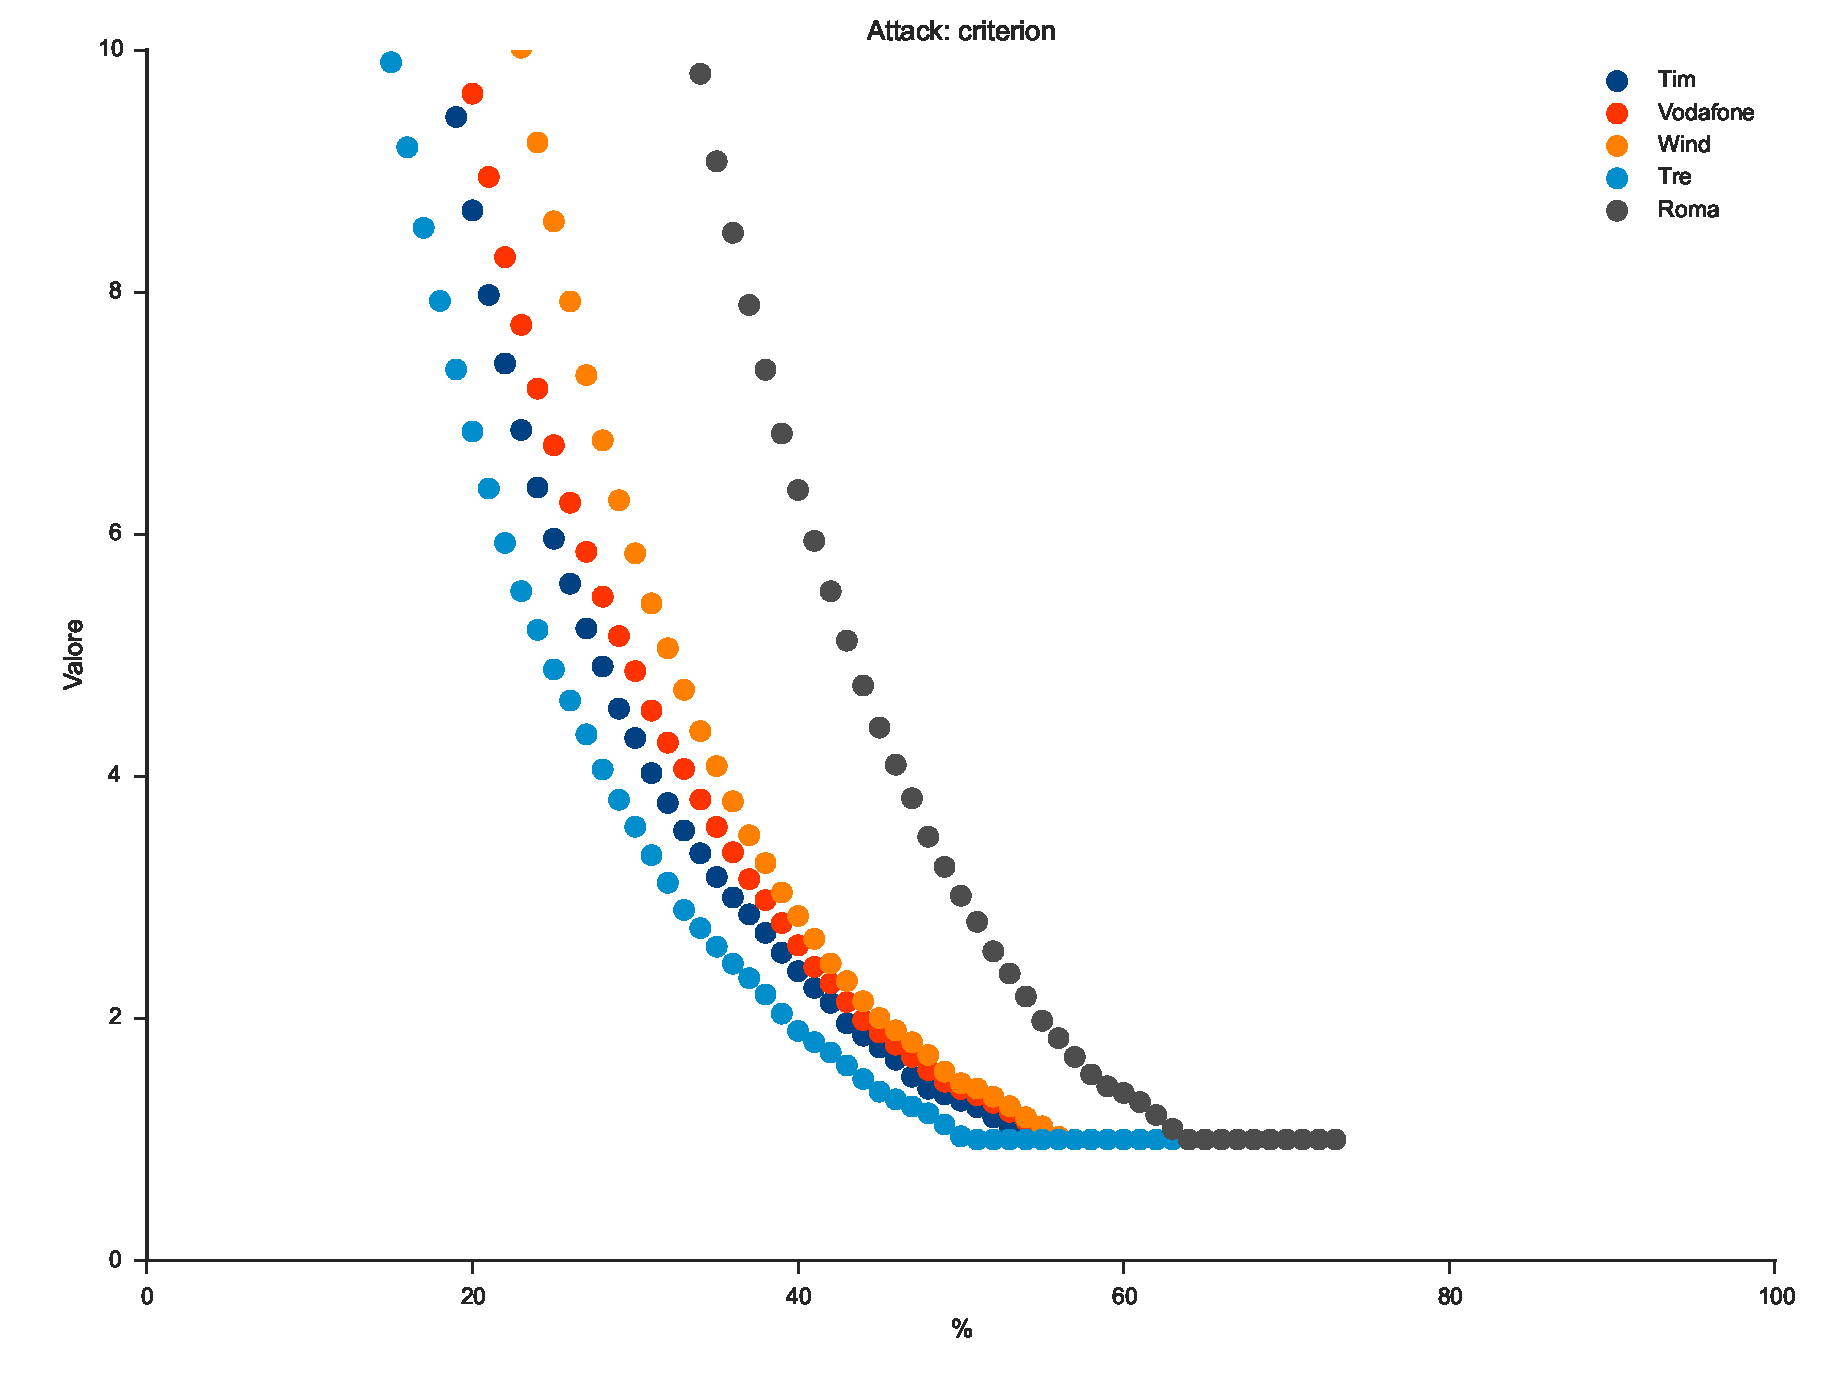
\includegraphics[width=0.47\textwidth]{./Immagini/Attack/gToolAttackc_Final}}
	\caption[Risultati attacco.]{Risultati per rimozione con massima efficienza}
	\label{fig:atak}
\end{figure}
\clearpage
\section{Conclusioni}
Come abbiamo visto, in regime di alta connettività dal punto di vista percolativo si notano poco le differenze tra reti generate secondo un modello scale-free o random. La differenza si nota quando il grado medio della rete è più basso. Per esempio una rete random con $\langle k \rangle \sim 2$ ha $f\sim 50\%$, mentre una rete scale free con stesso $\langle k \rangle$ ha $f\sim 80\%$. Una spiegazione qualitativa sta nel fatto che con una distribuzione del grado a legge di potenza, i nodi meno connessi sono in larga maggioranza, quindi è meno probabile che un attacco random riesca a destrutturare la rete, rispetto a un grafo che abbia una $P(k)$ poissoniana.

Uno studio percolativo su reti reali, quindi, non aiuta a identificare una eventuale invarianza di scala per reti molto grandi e connesse. Tuttavia può essere decisiva per reti più piccole, come piccole comunità, reti locali e alcuni ecosistemi: nonostante la bassa statistica, i comportamento di reti con pochi nodi possono essere distinti in maniera significativa da uno studio percolativo.

Nel caso di reti il cui funzionamento dipende dalla capacità dei nodi di gestire un certo carico, uno studio percolativo dovrebbe anche considerare l'eventualità che con la rimozione di alcuni nodi, altri vadano in sovraccarico e si scolleghino dalla rete, ovvero di un effetto cascata (Motter \citeyear{Motter2002}, Zhao \citeyear{Zhao2004} e \citeyear{Zhao2005}, Wang \citeyear{Wang2009}). È il caso delle reti comunicative, come quelle telefoniche cellulari analizzate o una ipotetica rete mesh costruita con i router WiFi, ma anche ovviamente reti di distribuzioni elettriche, ecc.

Una possibile interessante applicazione dei metodi e degli strumenti usati per analizzare la rete di antenne di Roma potrebbe essere lo studio di città molto più grandi e densamente popolate (come New York o Tokyo), ma servirebbero capacità di calcolo e di memoria molto più grandi di quelle a nostra disposizione. Un altro possibile studio potrebbe essere verificare la possibilità di creare una rete distribuita e aperta con i router WiFi.

%valutare se lasciare o rimuovere
Una rete di questo tipo sarebbe comunque un nuovo concetto di Internet, che potrebbe avere interessanti sviluppi su reti di altro tipo, per esempio sociali, correlate a essa.
% !TEX encoding = UTF-8
% !TEX TS-program = pdflatex
% !TEX root = ../Relazione.tex
% !TEX spellcheck = it-IT

%%%%%%%%%%%%%%%%%%%%%
\section{Conclusioni}
\label{sec:conc}
%%%%%%%%%%%%%%%%%%%%%

Come 

\newpage

% *****************************************************************
% Materiale finale
%******************************************************************
\clearpage
% !TEX encoding = UTF-8
% !TEX TS-program = pdflatex
% !TEX root = ../Articolo.tex
% !TEX spellcheck = it-IT

%*******************************************************
% Bibliografia
%*******************************************************
\nocite{*}
\printbibliography
\end{document}